\documentclass{beamer}
\usepackage{times}
\usepackage{tikz}
\usepackage{beamerthemesplit}
\usetheme{Antibes}
\usepackage{tcolorbox}

\title{The Security Framework of White-Box Cryptography Revisited}
\author{Yufeng Tang, Tao Sun, Zheng Gong\\ \url{cis.gong@gmail.com}}
\institute{\inst{1}{School of Computer Science, South China Normal University} \\ \inst{2}{Mobile Applications And Security Engineering Center of Guangdong Province}}

\date{\today}

\begin{document}

\frame
{
 \titlepage
}

\section[Outline]{}
\frame{\tableofcontents}

\section{White-box cryptography: background}
\frame{
\frametitle{Cryptography: the very beginning}
"Information theory is about communication in the presence of noise."
\begin{flushright}
-C. Shannon, 1948.\footnote{\scriptsize{\url{http://fab.cba.mit.edu/classes/S62.12/docs/Shannon_noise.pdf}}}
\end{flushright}

\begin{center}
\begin{tikzpicture}
    \node[anchor=south west,inner sep=0] (image) at (0,0) { 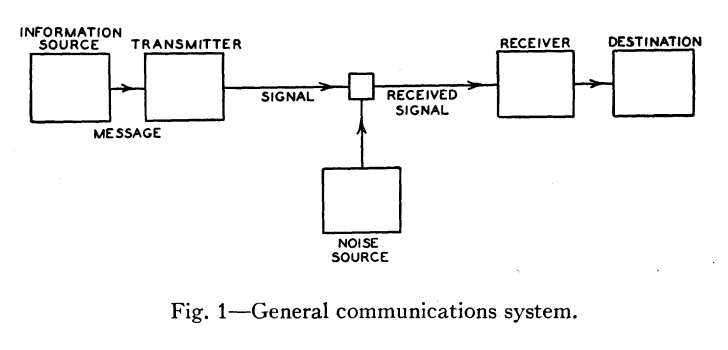
\includegraphics[width=8cm, height=4cm]{./pics/Shannon_GeneralCommunicationSystem.png}};

    %\begin{scope}[x={(image.south east)},y={(image.north west)}]
        %\draw[help lines,xstep=.1,ystep=.1] (0,0) grid (1,1);
        %\foreach \x in {0,1,...,9} { \node [anchor=north] at (\x/10,0) {0.\x}; }
        %\foreach \y in {0,1,...,9} { \node [anchor=east] at (0,\y/10) {0.\y}; }
        %\draw[green, ultra thick, rounded corners] (0.24,0.18) rectangle (0.50,0.32);
    %\end{scope}
\end{tikzpicture}
\end{center}
}

\frame{
\frametitle{Cryptography: an informal definition}
"Cryptography is about communication in the presence of adversaries."
\begin{flushright}
-R. Rivest
\end{flushright}

\begin{center}
\begin{tikzpicture}
    \node[anchor=south west,inner sep=0] (image) at (0,0) { 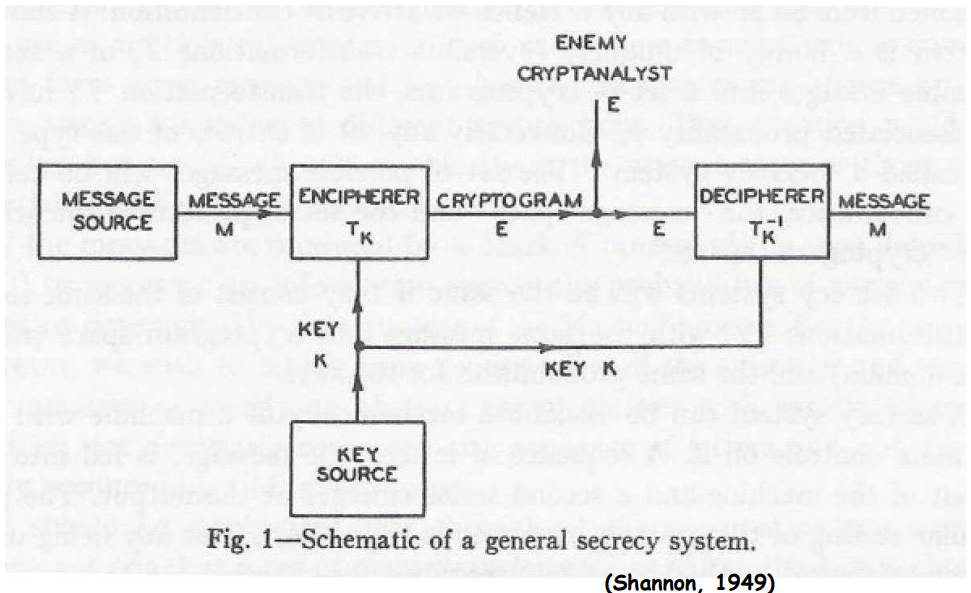
\includegraphics[width=8cm, height=5cm]{./pics/Shannon_GeneralSecrecySystem.png}};

    %\begin{scope}[x={(image.south east)},y={(image.north west)}]
        %\draw[help lines,xstep=.1,ystep=.1] (0,0) grid (1,1);
        %\foreach \x in {0,1,...,9} { \node [anchor=north] at (\x/10,0) {0.\x}; }
        %\foreach \y in {0,1,...,9} { \node [anchor=east] at (0,\y/10) {0.\y}; }
        %\draw[green, ultra thick, rounded corners] (0.24,0.18) rectangle (0.50,0.32);
    %\end{scope}
\end{tikzpicture}
\end{center}
}

\frame{
\frametitle{Define cryptography in ``a mathematically acceptable way"}
\textcolor{red}{``As a first step in the mathematical analysis of cryptography, it is necessary to idealize the situation suitably, and to define in a mathematically acceptable way what we shall mean by a secrecy system."}

\begin{flushright}
-C. Shannon, 1949. \footnote{{\scriptsize``Communication Theory of Secrecy Systems", Bell System Tech. J., vol. 28, pp. 656-715, Oct., 1949.}}
\end{flushright}
}

\frame
{
\frametitle{The Kerckhoffs' principle of cryptography}

\begin{columns}[c]
\column{.65\textwidth}
A cipher should be secure when the enemy cryptanalyst knows all details of the enciphering process and deciphering process except for the value of the secret key.

\begin{flushright}
- stated in 1881 by the Dutchman Auguste Kerckhoffs (1835-1903).
\end{flushright}
\begin{itemize}
\setlength{\itemsep}{12pt}
%\item Do not rely on keeping an algorithm secret.
%\item Publish an algorithm but keep the key secretly.
\item \textcolor{red}{Have some mathematical foundation for the belief that it will be hard to extract the key.}
\end{itemize}

\column{.35\textwidth}
\begin{figure}[htbp]
\centering
  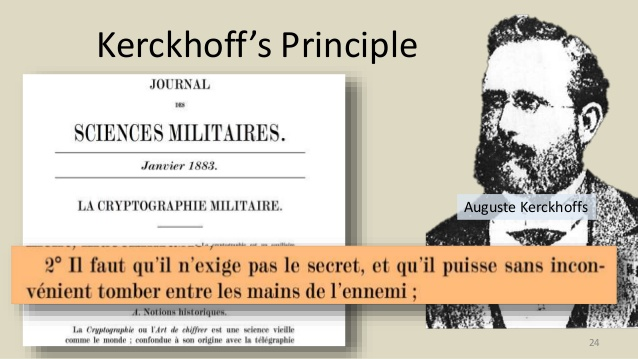
\includegraphics[width=4cm, height=3cm]{./pics/Kerckhoffs.jpg}
\end{figure}

\end{columns}
}

%\frame{
%\frametitle{The Kerckhoffs' principle of a secrecy system}
%A cipher should be secure when the enemy cryptanalyst knows all details of the enciphering process and deciphering process except for the value of the secret key.
%
%\begin{flushright}
%- stated in 1881 by the Dutchman Auguste Kerckhoffs (1835-1903).
%\end{flushright}
%
%
%\begin{center}
%\begin{tikzpicture}
%    \node[anchor=south west,inner sep=0] (image) at (0,0) { 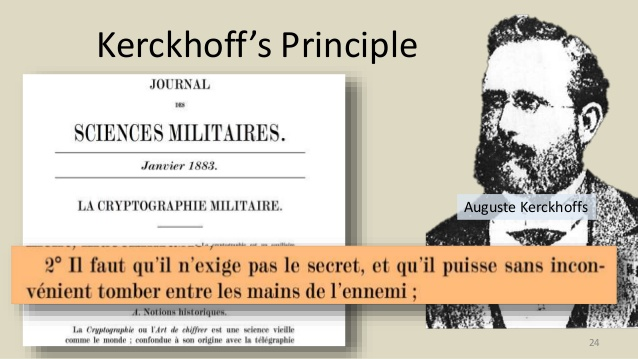
\includegraphics[width=6cm, height=4cm]{./pics/Kerckhoffs.jpg}};
%
%    %\begin{scope}[x={(image.south east)},y={(image.north west)}]
%        %\draw[help lines,xstep=.1,ystep=.1] (0,0) grid (1,1);
%        %\foreach \x in {0,1,...,9} { \node [anchor=north] at (\x/10,0) {0.\x}; }
%        %\foreach \y in {0,1,...,9} { \node [anchor=east] at (0,\y/10) {0.\y}; }
%        %\draw[green, ultra thick, rounded corners] (0.24,0.18) rectangle (0.50,0.32);
%    %\end{scope}
%\end{tikzpicture}
%\end{center}
%}

\frame{
\frametitle{The goal of modern cryptography}
\begin{itemize}
\item The goal of modern cryptography is to design, analysis, and implement a cryptosystem which obtains a mathematically acceptable security proofs.

\begin{itemize}
\item Confidentiality / Secrecy
\item Integrity
\item Authenticity
\item Availability
\end{itemize}

\item Thus provable security must be reduced on \textcolor{red}{an acceptable model!}
\begin{itemize}
\item Ideal cipher model
\item Random oracle model/Standard model
\item Indifferentiability model
\end{itemize}
\end{itemize}
}

\frame{
\frametitle{How to modeling attackers in cryptography}
\begin{center}
\begin{tikzpicture}
    %\node[anchor=south west,inner sep=0] (image) at (0,0) { 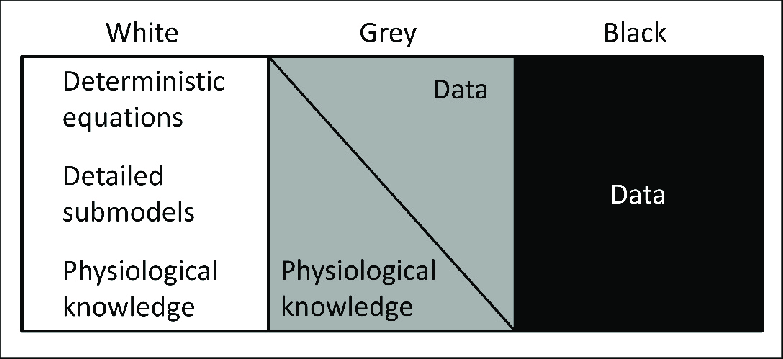
\includegraphics[width=6cm, height=4cm]{./pics/Illustration-of-the-concept-of-Black-White-Grey-box-modeling.png}};
    \node[anchor=south west,inner sep=0] (image) at (0,0) { 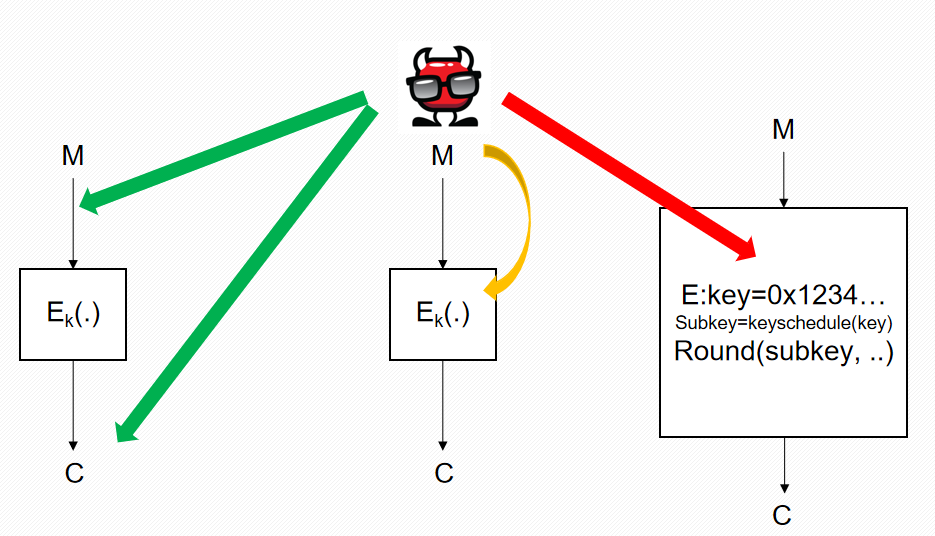
\includegraphics[width=7cm, height=4cm]{./pics/WBC_Model.png}};

    %\begin{scope}[x={(image.south east)},y={(image.north west)}]
        %\draw[help lines,xstep=.1,ystep=.1] (0,0) grid (1,1);
        %\foreach \x in {0,1,...,9} { \node [anchor=north] at (\x/10,0) {0.\x}; }
        %\foreach \y in {0,1,...,9} { \node [anchor=east] at (0,\y/10) {0.\y}; }
        %\draw[green, ultra thick, rounded corners] (0.24,0.18) rectangle (0.50,0.32);
    %\end{scope}
\end{tikzpicture}
\end{center}
}

\section{The security framework of WBC}
\subsection{Basic concepts of modeling}
\frame{
\frametitle{Black-box model}
\begin{itemize}
\item The adversary is able to know, choose or adaptively choose inputs and outputs of the function.

\item Given the black-box implementation of the function, the adversary aims to \textcolor{red}{recover the secret values} or to \textcolor{orange}{misbehave the function}.
\end{itemize}
}

\frame{
\frametitle{White-box model}
\begin{itemize}
\item Informally speaking, an adversary in \textcolor{red}{white-box model} can tamper, modify, manipulate all intermediate values and processes of the implementation of a secrecy system.
\item It can be looked as a superset of \textcolor{red}{black-box} and \textcolor{red}{grey-box} models.
\end{itemize}
}

\frame{
\frametitle{Grey-box model}
According to the black/white-box modeling, the grey-box adversary is able to
\begin{itemize}
\item know, choose or adaptively choose inputs and outputs of the function;

\item tamper, modify, manipulate intermediate values with specific (physical) knowledge.

\end{itemize}
}

\frame{
\frametitle{An illustration of the Black/White/Grey-box modeling}
\begin{center}
\begin{tikzpicture}
    \node[anchor=south west,inner sep=0] (image) at (0,0) { 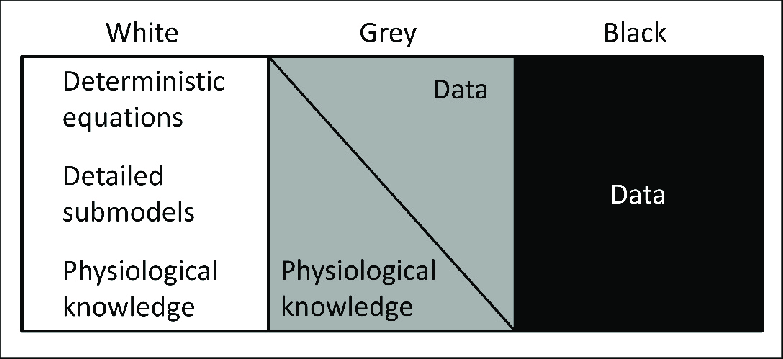
\includegraphics[width=9cm, height=4cm]{./pics/Illustration-of-the-concept-of-Black-White-Grey-box-modeling.png}};
    %\node[anchor=south west,inner sep=0] (image) at (0,0) { 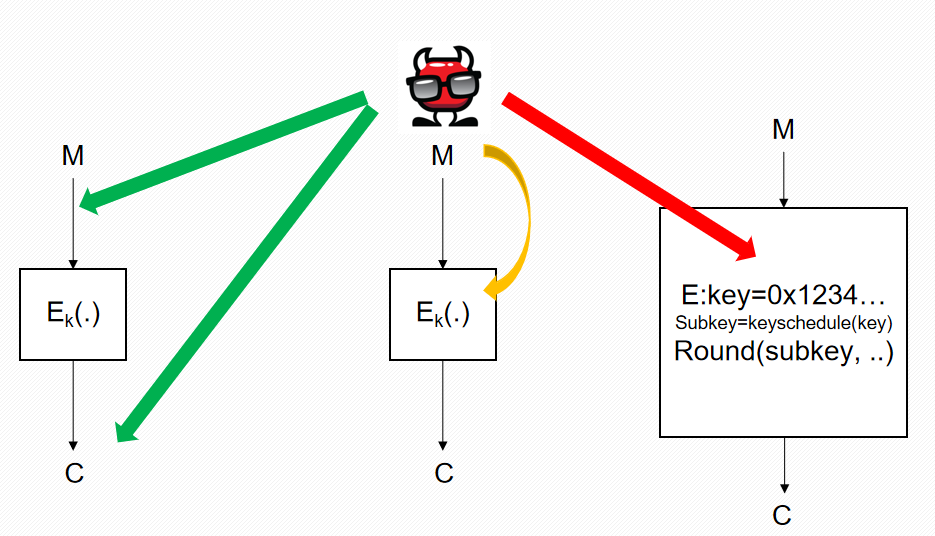
\includegraphics[width=7cm, height=4cm]{./pics/WBC_Model.png}};

    %\begin{scope}[x={(image.south east)},y={(image.north west)}]
        %\draw[help lines,xstep=.1,ystep=.1] (0,0) grid (1,1);
        %\foreach \x in {0,1,...,9} { \node [anchor=north] at (\x/10,0) {0.\x}; }
        %\foreach \y in {0,1,...,9} { \node [anchor=east] at (0,\y/10) {0.\y}; }
        %\draw[green, ultra thick, rounded corners] (0.24,0.18) rectangle (0.50,0.32);
    %\end{scope}
\end{tikzpicture}
\end{center}
}

\frame
{
\frametitle{A typical white-box block cipher in a nutshell}
\begin{figure}[htbp]
\centering
  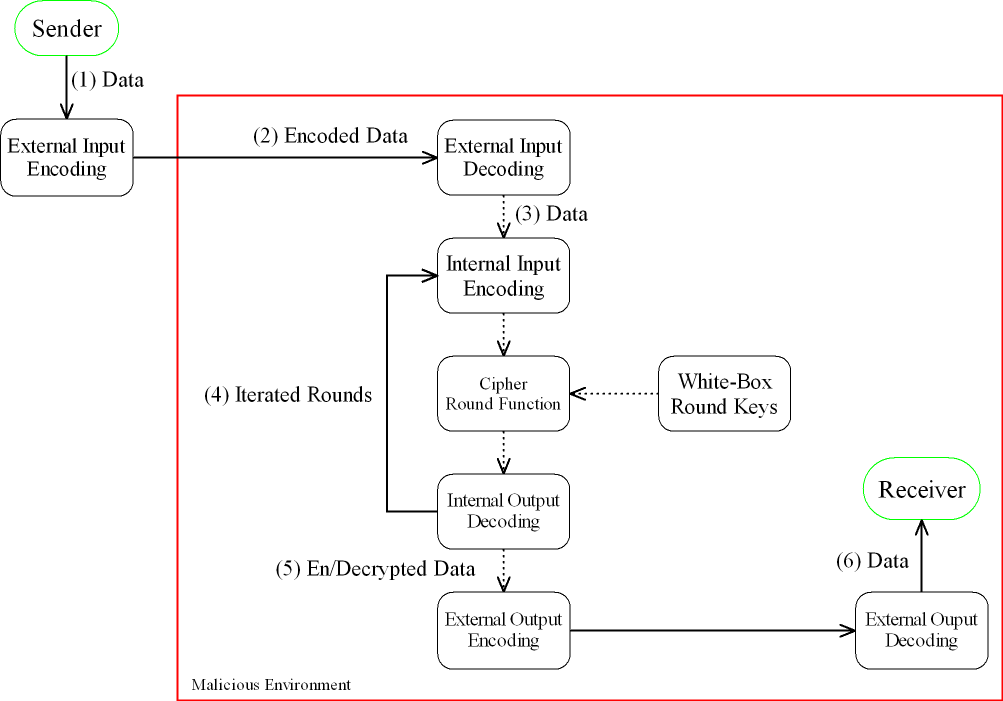
\includegraphics[width=8cm]{./pics/WBCrypto_Functional_Model.png}

\end{figure}

}

\frame
{
 \frametitle{WBC Implementations of DES/AES/SM4/... (All broken!)}
 \begin{itemize}
  \item Chow \textit{et al.} Tbox-based WBDES/AES, 2002
  \item Link and Neumann. Tbox-based WBTDES, 2005
  \item Bringer. Isomorphism of Polynomials, WBAES, 2006
  \item Xiao and Lai. 16-bit Tbox WBAES, 2009
  \item Xiao and Lai. Affine-function WBSM4, 2009
  \item Karroumi \textit{et al.} Dual-cipher WBAES, 2011
  \item Shi \textit{et al.} Tbox-based WBSHARK, 2013
  \item Luo \textit{et al.} ShiftRows table WBAES, 2014
  \item Su \textit{et al.} Random number WBCLEFIA, 2014
  \item Shi \textit{et al.} Dual-cipher WBSM4, 2015
  \end{itemize}
}

\frame
{
 \begin{itemize}
  \item Baek \textit{et al.} Larger Tbox WBAES, 2016
  \item Bai and Wu. Uncombinable encodings WBSM4, 2016
  \item Lee \textit{et al.} Masked WBAES, 2018
  \item Xu \textit{et al.} Obfuscated round boundaries WBAES/SM4, 2018
  \item Bai \textit{et al.} Affine-function WBAES, 2018
  \item Zhou \textit{et al.} Lightweight WBC, 2018
  \item Lv \textit{et al.} WB-KMAC, 2019
  \item Lee and Kim. Table redundancy WBAES, 2019
  \item Lee and Kim. Improved masked WBAES, 2020
  \item Yao and Chen. Random state WBSM4, 2020
  \item Yao \textit{et al.} Affine-function WBCLEFIA, 2020
  \item Yao \textit{et al.} Affine-function WBGIFT, 2021
 \end{itemize}
}

\frame
{
 \frametitle{Dedicated WBC Proposals}
 \begin{itemize}
  \item Biyukov \textit{et al.} ASASA structure, 2014
  \item Bogdanov and Isobe. SPACE, 2015
  \item Bogdanov and Isobe. SPNbox, 2016
  \item Fouque \textit{et al.} WhiteBlock, 2016
  \item Bai and Wu. AES-Like cipher, 2016
  \item Cho and Dinur. WEM, 2017
  \item Lin \textit{et al.} ASASASA structure, 2017
  \item Xu \textit{et al.}. AES-like cipher, 2017
  \item Shi \textit{et al.} SDSRS, 2020
  \item Kwon \textit{et al.} FPL, 2020
  \item Koike \textit{et al.} Galaxy, 2020
 \end{itemize}
}

\subsection{The proposed security notions and their problems}
%
%\frame{
%\frametitle{Chow \textit{et al.}'s definitions}
%In Chow \textit{et al.}'s seminal work on white-box AES implementations, they proposed some basic notions intuitively.
%\begin{itemize}
%\item White-box attack context
%\item White-box s
%\item White-box security metrics
%
%\end{itemize}
%}

\frame{
\frametitle{Basic security definitions for WBC}
\begin{definition}(\textcolor{red}{Secret key recovery (KR-Security)}). A white-box implementation of a key-instantiated block cipher $E_{k}$ (or $D_{k}$) is called \textit{KR-insecure} if an attacker extracts the secret key $k$ and furthermore has access to the plaintext $P$.
\end{definition}

\begin{definition}
(\textcolor{red}{White-box key recovery (WBKR-Security)}). A white-box implementation of an encoded version of a key-instantiated block cipher $E_{k}$ (or $D_{k}$) is called \textit{WBKR-insecure} if the attacker extracts the secret key $k$ and the inverse mappings of the applied external encodings.
\end{definition}
}

\frame{
\frametitle{Basic security definitions for WBC (Chow \textit{et al.})}
\begin{itemize}
\item In SAC 2002, the security notions have  been informally described for white-box cryptography by Chow \textit{et al.}. First the key recovery problem is informally defined by \textcolor{red}{the weak white-box security} (which equals to \textcolor{red}{KR-Security})
\end{itemize}

\begin{center}
\begin{tikzpicture}
    \node[anchor=south west,inner sep=0] (image) at (0,0) { 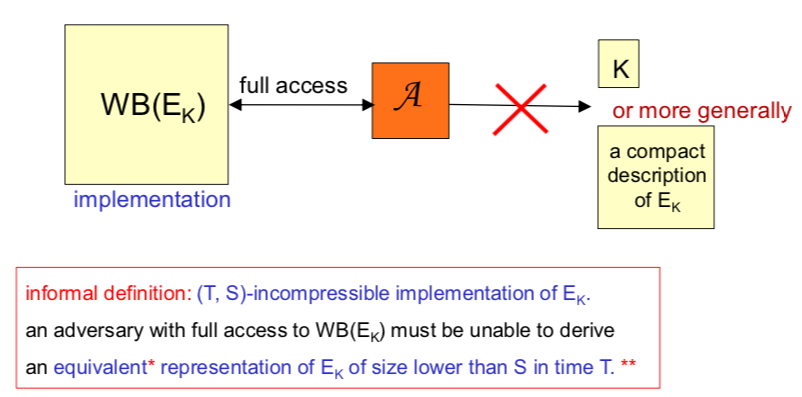
\includegraphics[width=8cm, height=4cm]{./pics/weak_white_box_security.png}};

    \begin{scope}[x={(image.south east)},y={(image.north west)}]
        %\draw[help lines,xstep=.1,ystep=.1] (0,0) grid (1,1);
        %\foreach \x in {0,1,...,9} { \node [anchor=north] at (\x/10,0) {0.\x}; }
        %\foreach \y in {0,1,...,9} { \node [anchor=east] at (0,\y/10) {0.\y}; }
        \draw[red, thin, rounded corners] (0.85,0.7) circle (1.2cm);
    \end{scope}
\end{tikzpicture}
\end{center}
}

\frame{
\frametitle{Basic security definitions for WBC (Biryukov \textit{et al.})}
\begin{itemize}
\item For more general security, \textcolor{red}{the strong white-box security} has been defined by [Biryukov \textit{et al.} 2014] (which connects to \textcolor{red}{KR/WBKR-Security})
\end{itemize}

\begin{center}
\begin{tikzpicture}
    \node[anchor=south west,inner sep=0] (image) at (0,0) { 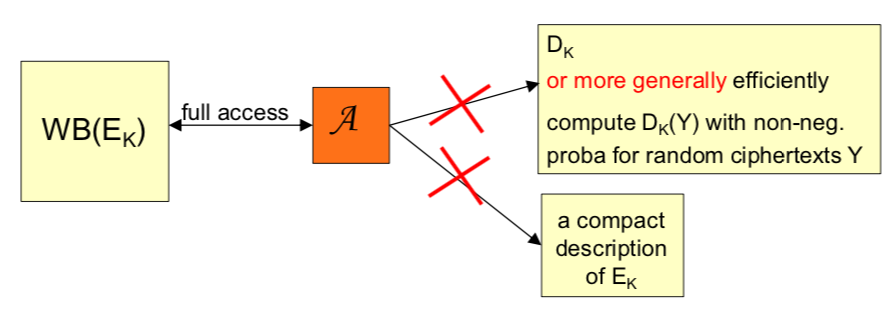
\includegraphics[width=10cm, height=4cm]{./pics/strong_white_box_security.png}};

    %\begin{scope}[x={(image.south east)},y={(image.north west)}]
        %\draw[help lines,xstep=.1,ystep=.1] (0,0) grid (1,1);
        %\foreach \x in {0,1,...,9} { \node [anchor=north] at (\x/10,0) {0.\x}; }
        %\foreach \y in {0,1,...,9} { \node [anchor=east] at (0,\y/10) {0.\y}; }
        %\draw[green, ultra thick, rounded corners] (0.24,0.18) rectangle (0.50,0.32);
    %\end{scope}
\end{tikzpicture}
\end{center}
}


\frame{
\frametitle{The problems of the weak/strong white-box security}
\begin{itemize}
\item It only works for white-box encryption/decryption, while does not suitable for \textcolor{red}{MAC/signature}.

\item ``A \textcolor{red}{compact} description of $E_{k}$/$/D_{k}$", it is very hard to measure security under this informal definition.
\end{itemize}
}

\frame{
\frametitle{The negative results on virtual black-box property (VBBP)}
\begin{itemize}
\item At Crypto 2001, Barak \textit{et al.} provided an insight on the impossibility of code obfuscation for \textcolor{red}{generic programs}.
\item \textcolor{red}{The virtual black-box property (VBBP)} has been proposed for defining the ideal code/program obfuscation.
\item The negative results are given by counterexamples that cannot satisfy the virtual black-box property (VBBP) in any circumstance.
\end{itemize}
}

\frame{
\frametitle{Recall the definitions of VBBP [Saxena2009] (1)}
\textbf{Correctness.}{$\mathcal{O}$ is an obfuscator for a polynomial time function $Q$ if the follow properties hold.}
\begin{enumerate}

\item \textit{(\textcolor{red}{Functionality})}. $\forall k, \forall (q,a)\in \mathcal{K}^{k}_{Q}\times \mathcal{I}^{k}_{Q}:\textmd{Pr}[\mathcal{O}(Q,k)(a) \neq Q [k](a)]\leq negl(k)$

\item \textit{(\textcolor{red}{Polynomial slowdown and expansion})}. $\exists p \in \mathbb{P}, \forall k, \forall q \in \mathcal{K}^{k}_{Q}:$
\begin{itemize}
    \item $|\mathcal{O}(Q, q)| \leq p(k)$;
    \newline
    \item $\forall a: Q[q](a) \leq t \rightarrow \mathcal{O}(Q,q)(a) \leq p(t)$
\end{itemize}
\end{enumerate}
}

\frame{
\frametitle{Recall the definitions of VBBP [Saxena2009] (2)}
\begin{itemize}
\item Let $Q[q]$ be a random instance of a polynomial Turing machine family (PTMF) $Q$ under key $q$.

\item The VBBP requires that whatever information that adversary $\mathcal{A}$ extracts from $\mathcal{O}(Q,q)$, simulator $\mathcal{S}$ can also extract with black-box access to $Q[q]$.

\item The existing notions of VBBP can be categorized in the following two directions.
\begin{itemize}
\item \textit{Predicate VBBP}

\item \textit{Indistinguishability}
\end{itemize}

\end{itemize}

[Saxena 2009] noted that \textit{Predicate VBBP(pvbbp)} is too weak for practice, on the other hand \textit{Indistinguishability} is too strong to be achievable.
}

\frame{
\frametitle{Recall the definitions of VBBP [Saxena2009] (3)}

\textbf{Soundness.}{$\mathcal{O}$ is sound if at least one of the following properties holds.}
\begin{enumerate}
\item \textit{Predicate VBBP:}$\forall A\in \mathbb{PPT}, \exists S \in \mathbb{PPT}: Adv_{A, S, \mathcal{O}, Q}^{pvbbp} \leq negl(k)$, where \\ $Adv_{A, S, \mathcal{O}, Q}^{pvbbp}(k) =|\textmd{Pr}_{q \xleftarrow{R} \mathcal{K}^{k}_{Q}}[A^{Q[q]}(1^{k},\mathcal{O}(Q,q))=1 \wedge S^{Q[q]}(1^{k})\neq 1]|$.

\item \textit{Indistinguishability:} $\forall A\in \mathbb{PPT}, \exists S \in \mathbb{PPT}: Adv_{A, S, \mathcal{O}, Q}^{ind} \leq negl(k)$, where \\ $Adv_{A, S, \mathcal{O}, Q}^{ind}(k) =|\textmd{Pr}_{q \xleftarrow{R} \mathcal{K}^{k}_{Q}}[A^{Q[q]}(1^{k},\mathcal{O}(Q,q))=1 \wedge A^{Q[q]}(1^{k}, S^{Q[q]}(1^{k}))\neq 1]|$.
\end{enumerate}


}

\frame{
\frametitle{Saxena \textit{et al.}'s WBC proposal}
\begin{enumerate}
\item Encryption: $E[k]:(m, r) \mapsto (H(\hat{e}(\textcolor{red}{k}^{r}, g)\oplus m), g^{r}) \mapsto (c_{1}, c_{2})$

\item Decryption:$D[k]: (c_{1}, c_{2}) \mapsto H(\hat{e}(c_{2}, k))\oplus c_{1} \mapsto m$

\item White-box encryption: Let $y = \textcolor{red}{\hat{e}(k, g)}$, $\mathcal{O}(E[k]): (m, r) \mapsto (H( \textcolor{red}{y}^{r}) \oplus m, g^{r}) \mapsto (c_{1}, c_{2})$\newline

\end{enumerate}


The problem:
\begin{itemize}
\item only CPA-security, to achieve CCA-Security requires MAC on message. (\textcolor{red}{which means another authenticated key!})

\item Black-box security can be reduced to the discrete logarithm problem (\textcolor{red}{$k^{r}$}), whilst white-box security is the pairing inversion problem. ($y = \hat{e}(\textcolor{red}{k}, g)$)
\end{itemize}
}


\subsection{Application-oriented security notions}

\frame{
\frametitle{Chow \textit{et al.}'s White-box metrics}
[CEJO2002] introduced a few metrics that try to measure the achieved level of white-box security for LUT-based implementations.
\begin{itemize}
\item \textcolor{red}{White-box diversity}: how many distinct ways a particular unencoded LUT can be encoded. For key-dependent LUTs, the variation of the embedded key-material needs to be considered.
\[\mathcal{T'} = g \circ T \circ f, \textmd{WB-div}=\#g \times \#T \times \#f \]

\item \textcolor{red}{White-box ambiguity}: how many distinct ways a specific encoded LUT can be interpreted.
\[\textmd{WB-amb{T'} = \textmd{WB-div}(T')/\#T'}\]

\item \textcolor{red}{Local security}: Indistinguishability on $\mathcal{T'}$ with different keys and encodings.
\end{itemize}
}

\frame{
\frametitle{The problems of Chow \textit{et al.}'s White-box metrics}
\begin{itemize}
\item White-box diversity/ambiguity and local security cannot imply to KR/WBKR-security.

\item The increase number of white-box diversity/ambiguity cannot be related to the achieved security level.

\item It is very hard to accurately count white-box diversity/ambiguity due to the bijection restriction.

\end{itemize}

}

\frame
{
\frametitle{Tamper resistance for DRM}

\begin{itemize}
\item Michiels and Gorissen [DRM'07] proposed a method to protect the integrity of software which depends on the correct operation of the white-box implementation of a block cipher.
%\item If an attacker modifies the software, the white-box implementation stops decrypting/encrypting properly.
\begin{tcolorbox}[title=security goal]
\item The proposed method assume that it is the goal of an attacker to \textcolor{red}{modify} the protected software without losing the ability to decrypt/encrypt properly.
\end{tcolorbox}
\end{itemize}

}

\frame{

\frametitle{White-box security objectives}
For the application in which a white-box implementation is deployed, [Delerabl$\acute{e}$e \textit{et al.} 2013] discussed the following security objectives.

\begin{itemize}
\item One-wayness: implies the strong white-box security

\item Incompressibility: prevents the a functionally equivalent deduction \textcolor{red}{with a significantly smaller memory footprint}.

\item Traceability: make a white-box implementation traceable.

\end{itemize}

}

\frame{
\frametitle{Space-hard ciphers:SPACE}
\begin{itemize}
\item In CCS 2015, Bogdanov and Isobe proposed a family of white-box block cipher \textcolor{red}{SPACE} with several novel features.
\begin{itemize}
\item SPACE-hardness: The implementation of $E_{K}$ is $(M, Z)$-space hard if it is infeasible to en/decrypt any randomly drawn plain/ciphertext with probability of more than $2^{-Z}$ given any code (LUT) of size less than $M$.\newline

\item Strong $(M, Z)-Space hardness$: existential possibility version of $(M, Z)-Space hardness$.
\end{itemize}
\end{itemize}



}

\frame{
\frametitle{Space-hard ciphers:SPACE}
\begin{center}
\begin{tikzpicture}
    \node[anchor=south west,inner sep=0] (image) at (0,0) { 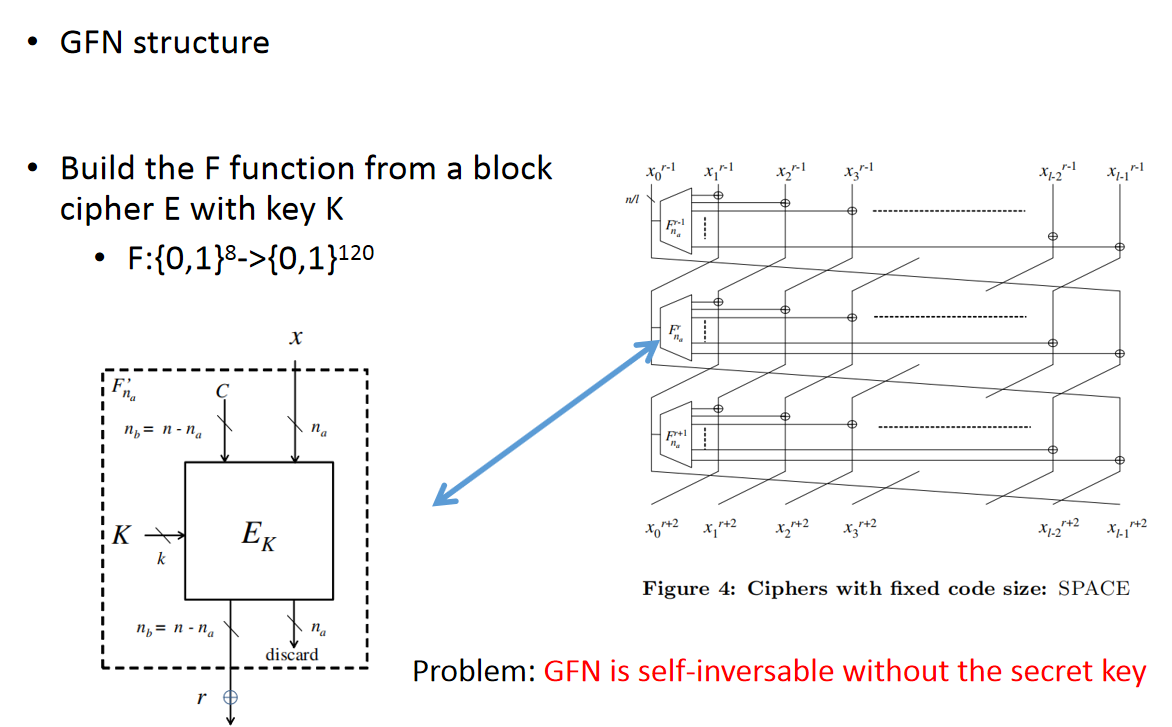
\includegraphics[width=8cm, height=5.5cm]{./pics/SPACE.png}};

    %\begin{scope}[x={(image.south east)},y={(image.north west)}]
        %\draw[help lines,xstep=.1,ystep=.1] (0,0) grid (1,1);
        %\foreach \x in {0,1,...,9} { \node [anchor=north] at (\x/10,0) {0.\x}; }
        %\foreach \y in {0,1,...,9} { \node [anchor=east] at (0,\y/10) {0.\y}; }
        %\draw[green, ultra thick, rounded corners] (0.24,0.18) rectangle (0.50,0.32);
    %\end{scope}
\end{tikzpicture}

\end{center}

}


\frame{
\frametitle{Space-hard ciphers:SPNBox}
In Asiacrypt 2016, Bogdanov and Isobe proposed \textcolor{red}{SPNBox}, which can be looked as the SPN version of SPACE.
\begin{center}
\begin{tikzpicture}
    \node[anchor=south west,inner sep=0] (image) at (0,0) { 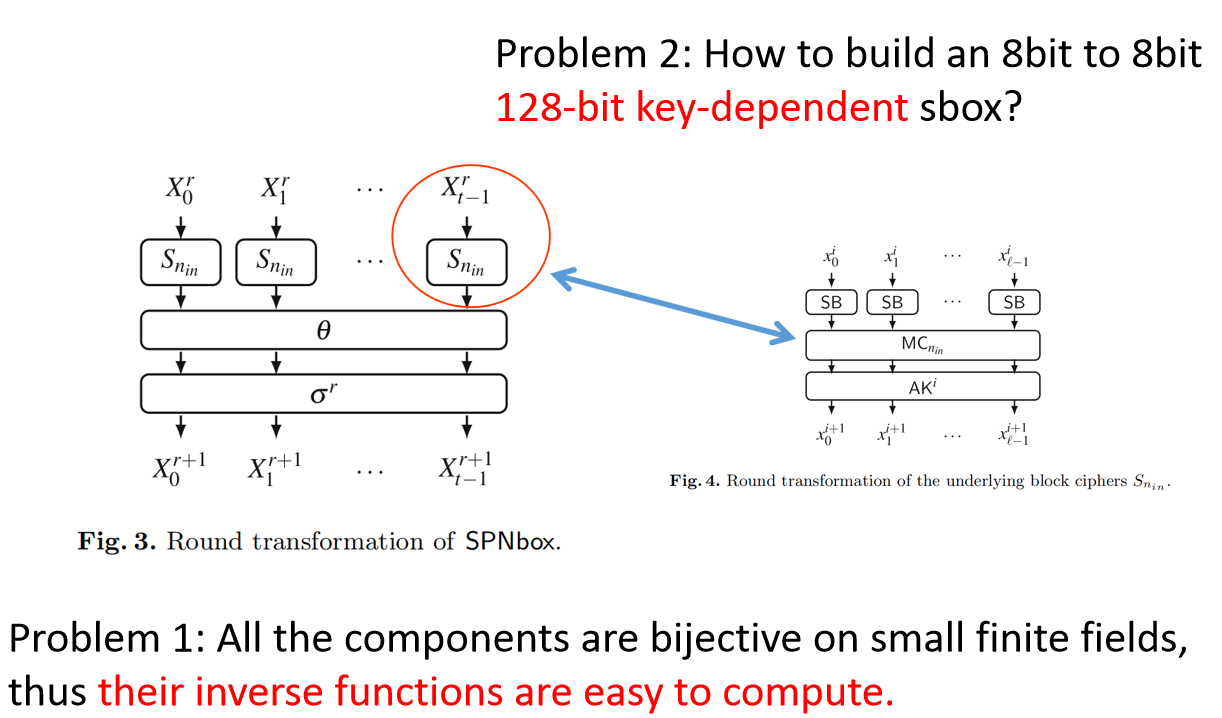
\includegraphics[width=8.5cm, height=5.5cm]{./pics/SPNBox.png}};

    %\begin{scope}[x={(image.south east)},y={(image.north west)}]
        %\draw[help lines,xstep=.1,ystep=.1] (0,0) grid (1,1);
        %\foreach \x in {0,1,...,9} { \node [anchor=north] at (\x/10,0) {0.\x}; }
        %\foreach \y in {0,1,...,9} { \node [anchor=east] at (0,\y/10) {0.\y}; }
        %\draw[green, ultra thick, rounded corners] (0.24,0.18) rectangle (0.50,0.32);
    %\end{scope}
\end{tikzpicture}

\end{center}

}

\frame
{
\frametitle{The problems of Space-hard ciphers}
\begin{itemize}
\item \textcolor{red}{Performance}: The costs of LUTs and computation are higher than CEJO-like constructions.\newline

\item \textcolor{red}{Weak WBC}: only achieves the weak white-box security (add encodings might be helpful but even worse on performance).

\item \textcolor{red}{Accuracy of space-hardness}: For example, if give 1000 bytes out of a 1024 bytes LUT, does attacker need to exhaustively search the remain 24 bytes?

\item \textcolor{red}{Compatibility}: only works for new designs (especially block ciphers).
\end{itemize}
}

\frame{
\frametitle{Bock \textit{et al.}'s white-box security with hardware/application-binding}
In Asiacrypt 2020 and CHES 2020, Bock \textit{et al.} proposed a white-box security key derivation function with \textcolor{red}{hardware/application-binding}, and then built a white-box payment application on it.

\begin{center}
\begin{tikzpicture}
    \node[anchor=south west,inner sep=0] (image) at (0,0) { 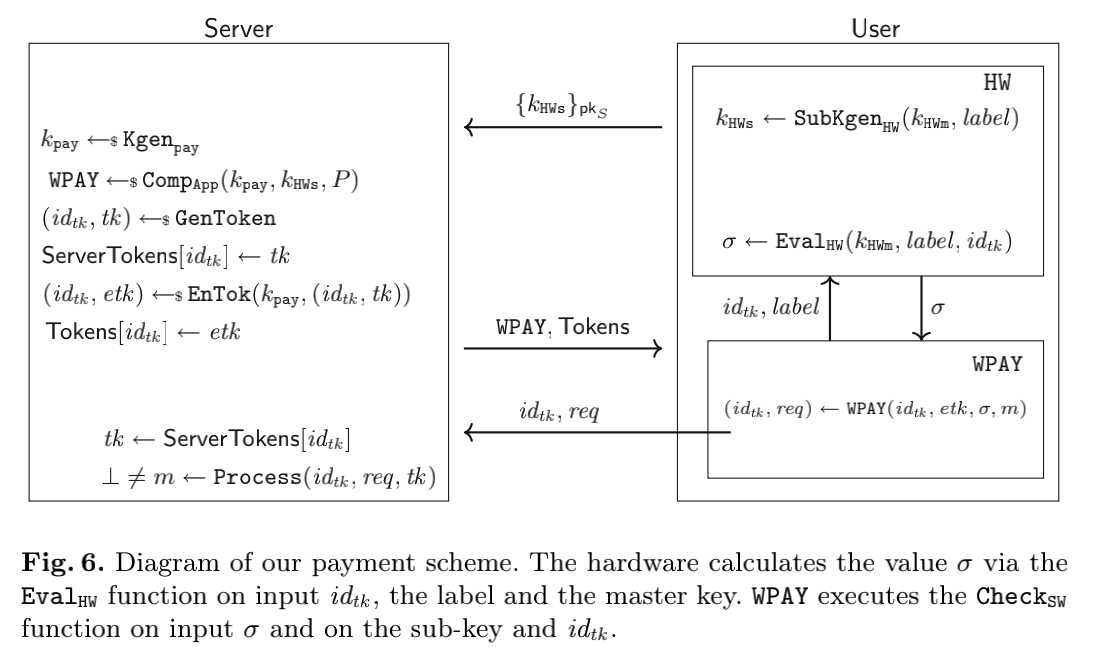
\includegraphics[width=8cm, height=5cm]{./pics/WKDF.png}};

    %\begin{scope}[x={(image.south east)},y={(image.north west)}]
        %\draw[help lines,xstep=.1,ystep=.1] (0,0) grid (1,1);
        %\foreach \x in {0,1,...,9} { \node [anchor=north] at (\x/10,0) {0.\x}; }
        %\foreach \y in {0,1,...,9} { \node [anchor=east] at (0,\y/10) {0.\y}; }
        %\draw[green, ultra thick, rounded corners] (0.24,0.18) rectangle (0.50,0.32);
    %\end{scope}
\end{tikzpicture}

\end{center}
}

\frame{
\frametitle{The problems of Bock \textit{et al.}'s hardware/application bound white-box security}
\begin{itemize}
\item It is not truly white-box security anymore if the precondition is a secure hardware. It becomes trusted computing.\newline

\item How to achieve hardware-binding is missing in the paper, the authors suggest using Android Keystore (which is insecure when it is rooted.)\newline

\item \textcolor{red}{If we already had a trusted hardware, why we need white-box cryptography? (e.g., using TEE is a better choice)}
\end{itemize}
}

\section{Adaptive SCA model and its applications}
\subsection{Adaptive SCA model}

\frame{
\frametitle{SCA Model on WBC}
In CHES 2016, Bos \textit{et al.} proposed that WBC can be attacked by SCA techniques under grey-box model.
\begin{itemize}
\item Using SCA techniques can \textcolor{red}{avoid the reverse engineering work}, which always be time-costly in practice.

\item For a WBC implementation, DCA/DFA exploits the first and the last rounds respectively.
\end{itemize}
}

\frame
{
	\frametitle{Revisiting DFA/DCA and their countermeasures}
	\begin{itemize}
		\item DFA
        \begin{enumerate}
        \item Getting a fault-free ciphertext.
	    \item Injecting the faults and collecting the faulty ciphertexts.
	    \item Building a model and performing an analysis between the fault-free and faulty ciphertexts to find the key by solving equations.
        \end{enumerate}
        \item DCA
        \begin{enumerate}
	    \item The software counterpart of the Differential Power Analysis attack. 
	    \item Instead of physical measurements, DCA employs instrumentation tools like Valgrind, or PIN to capture the  memory traces.
	    \item A statistical analysis between the collected traces and the prediction of a key-dependent intermediate value.
        \end{enumerate}
    \end{itemize}

    Their countermeasures:   
	\begin{itemize}
		\item The obfuscation and the runtime protections (e.g., the desynchronization, virtual machine, dummies, and duplicates).
		\item The well-known SCA countermeasures (e.g., redundancy, masking, and shuffling).
	\end{itemize}
}

\frame
{
	\frametitle{The Adaptive Side-Channel Analysis Model on WBC}
	Although some improved white-box schemes can prevent the generalized SCA attacks (e.g., DFA and DCA), a white-box adversary can combine the powerful ability in the \textit{white-box context} with the technique of well-studied SCA attacks.
	\\[2ex]
	An \textbf{Adaptive Side-Channel Analysis} is an SCA attack scenario in which the attacker has the ability
	to make her choice of the inputs to the cryptographic function based on the previous chosen plaintexts queries and their corresponding intermediates.
}

\frame
{
	\frametitle{The abilities of adaptive SCA attacker}
	\begin{itemize}
		\item (For choosing plaintexts.) The adversary has in-depth reverse engineering and cryptographic skills to de-obfuscate the white-box implementation.
		\item (For practical SCA attack.) The adversary is capable of the generalized SCA attacks (e.g., DFA and DCA) on the white-box implementation.
	\end{itemize}
	This is assumed that the adversary has the identical abilities to a white-box attacker when querying the cryptographic function for choosing inputs/plaintexts. E.g., the adversary can deconstruct step by step the algorithms and collect/tamper any intermediate values before the SCA attack.
}

\frame
{
	\frametitle{The steps of adaptive SCA attack}
	\begin{itemize}
		\item The adversary de-obfuscates the white-box implementation with reverse engineering effort and therefore exposes the intellectual property.
		\item The adversary collects the target inputs/plaintexts by analyzing the intermediate values of the pinpointed sub-function.
		\item The adversary mounts SCA attacks on the white-box implementation with the chosen inputs/plaintexts.
	\end{itemize}
}


\subsection{Adaptive DCA on Improved Masking WBAES}

\frame
{
	\frametitle{Improved Masking Method for Protecting Against DCA}
	Improved masking method [Lee \textit{et al.} 2020] applies the masking technique to the key-dependent intermediate value. Such scheme adds the random masks on the $Ty_i$ outputs and encodes the masked values and the masks used.
	\\[2ex]
	The unmasking is designed to combine with input decoding of the second round.
}

\frame
{
	\frametitle{\textit{TypeII\_MO} table}
	Masks are randomly picked for each input, and the $8\times 8$ linear transformations are applied to the mask in \textit{TypeII\_MO} table.
	\begin{figure}
		\centering
		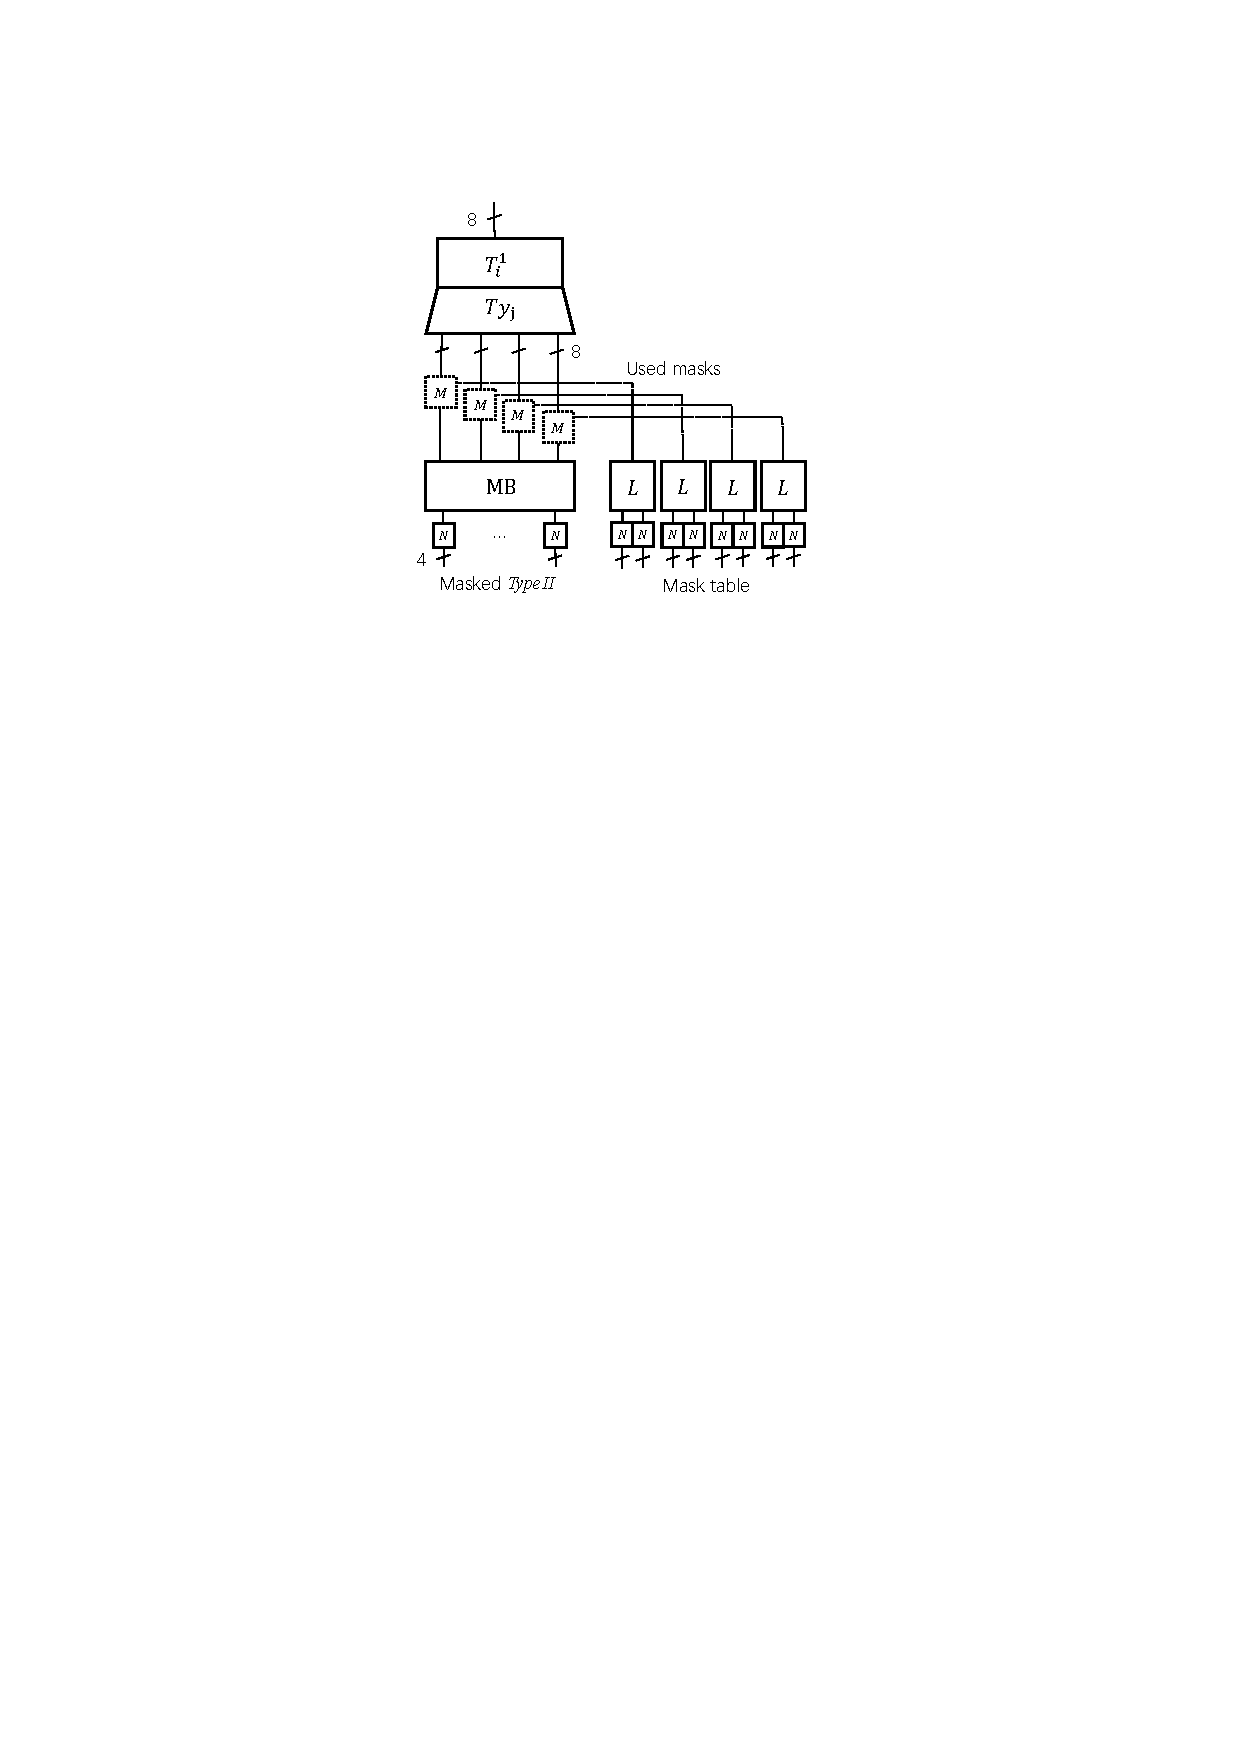
\includegraphics[width=5cm]{./pics/IIMO.pdf}
		\caption{\textit{TypeII\_MO} table.}
	\end{figure}
}

\frame
{
	\frametitle{\textit{TypeII\_MIMO} table}
	The encoded masked 1-st round output and the mask are combined by XOR to unmask in the input decoding phase of the second round.
	\begin{figure}
		\centering
		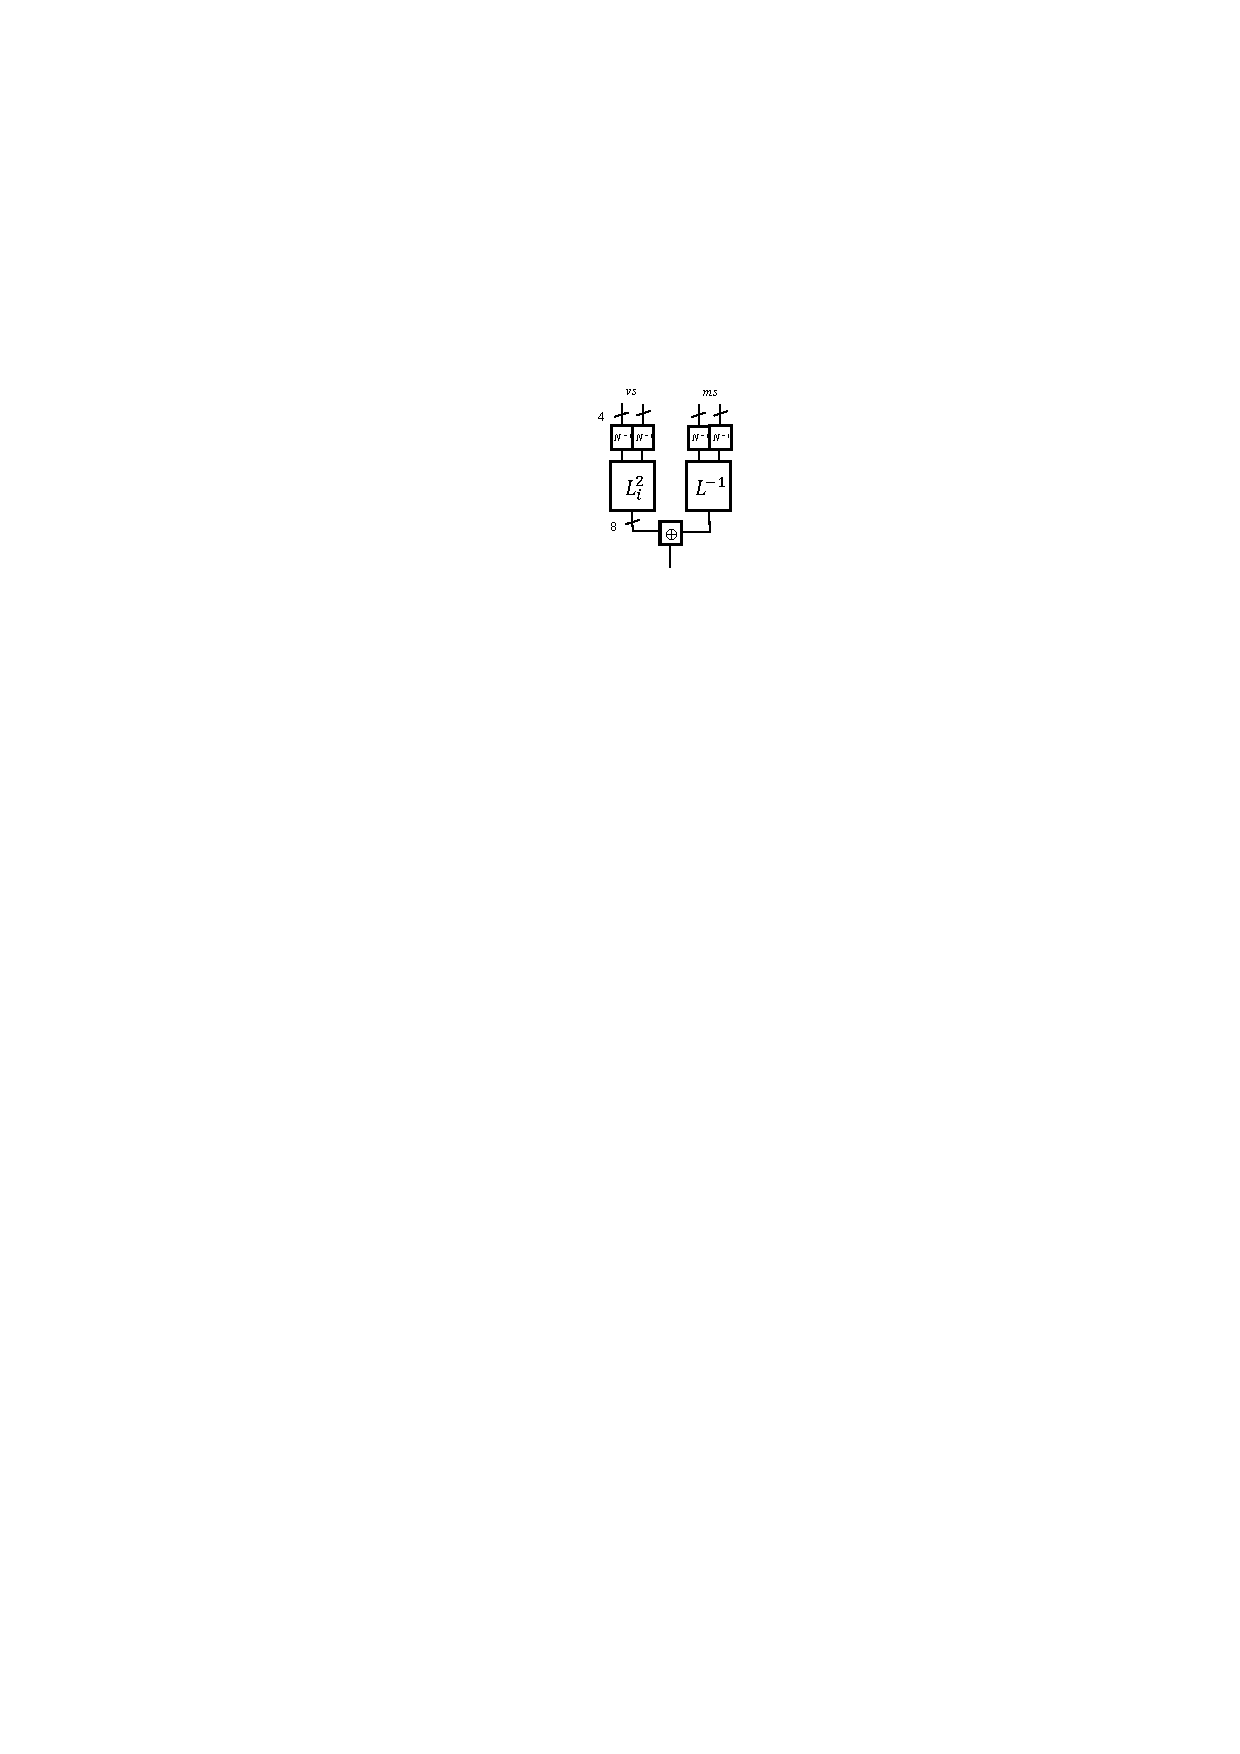
\includegraphics[width=3.0cm]{./pics/IIMIMO.pdf}
		\caption{\textit{TypeII\_MIMO} table.}
	\end{figure}
}

\frame
{
	\frametitle{DCA on Improved Masking Method}
	DCA fails to analyze the correlation between intermediate and hypothesis values.
	\begin{itemize}
		\item The mask is selected uniformly at random, and is independent with the input and key.
		\item The intermediates in the first round are all masked, and the unmasking is combined with the input decoding phase of the LUT in the second round.
	\end{itemize}
}

\frame
{
	\frametitle{Adaptive DCA against Improved Masking Method}
	\begin{figure}
		\centering
		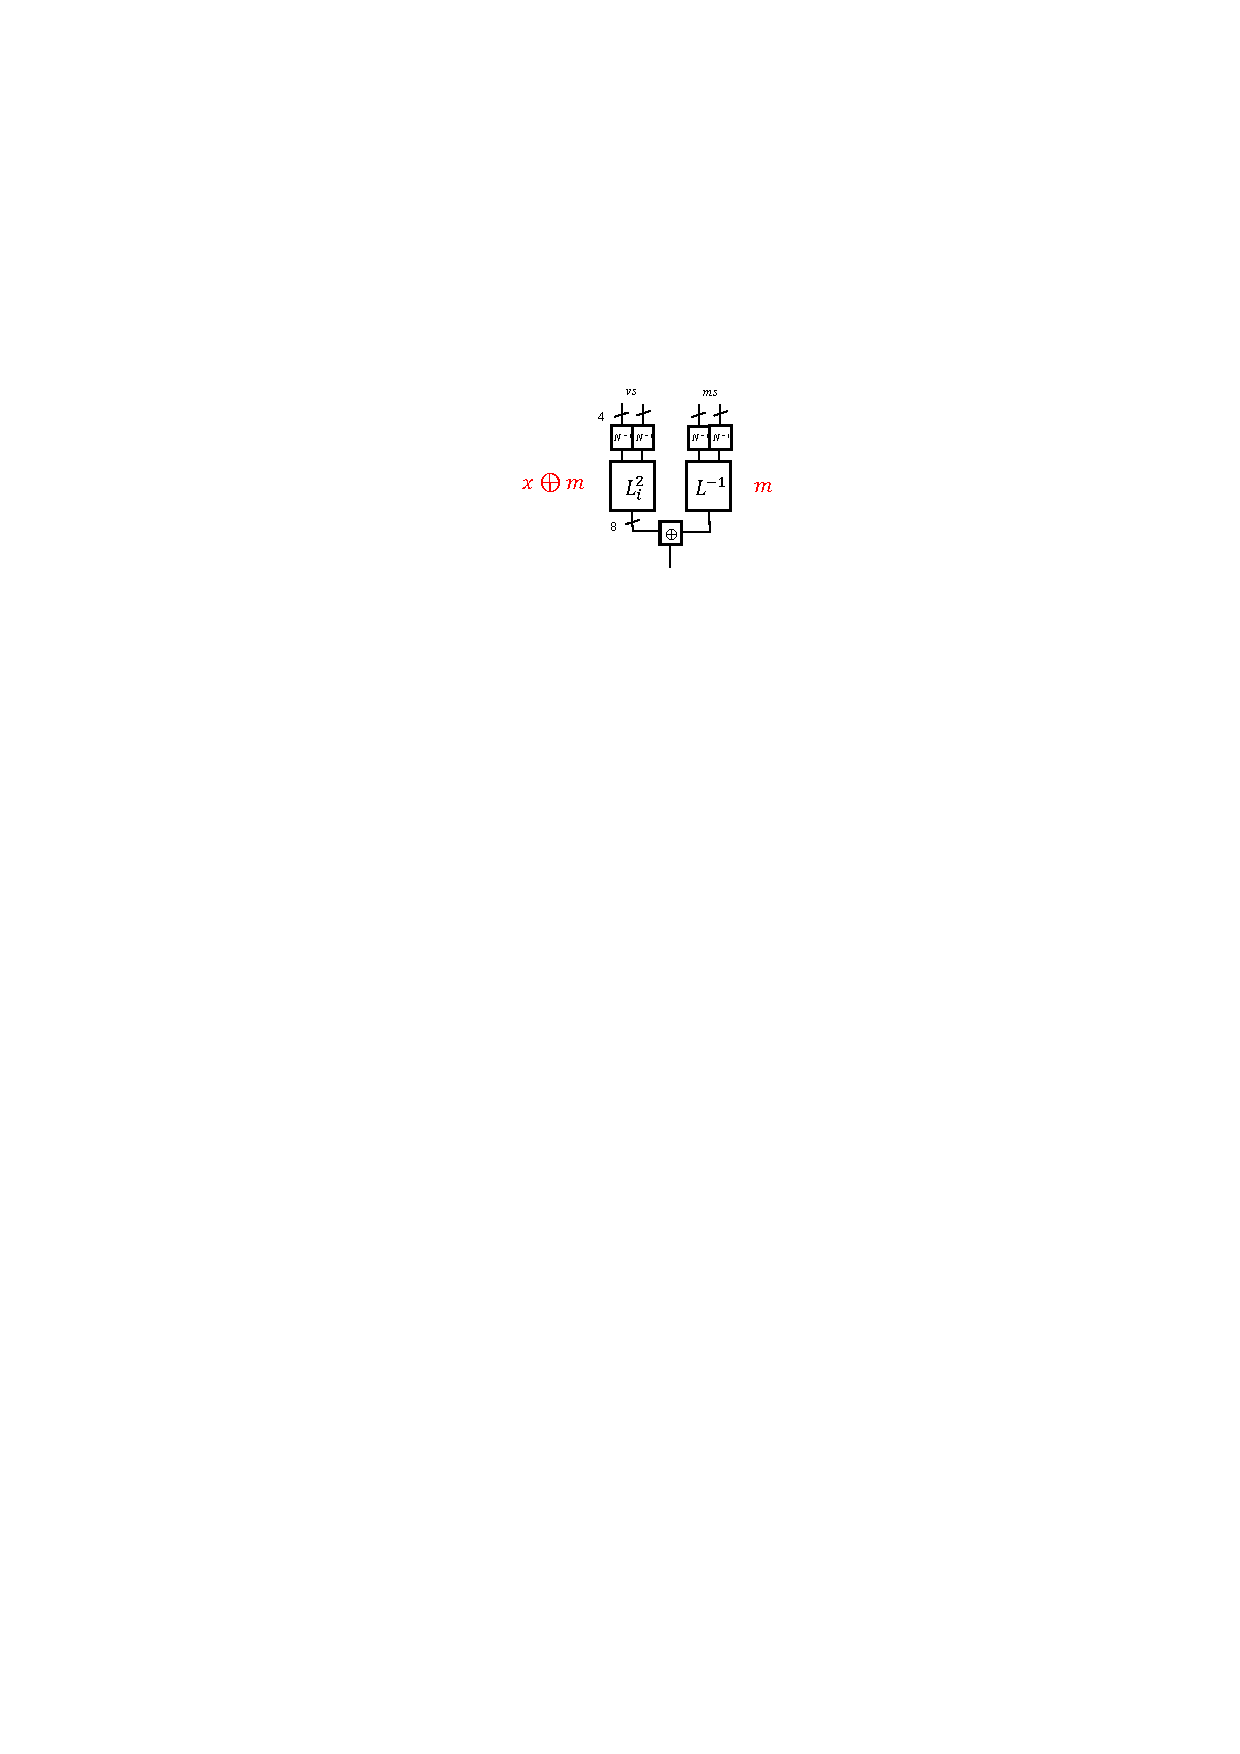
\includegraphics[width=3.5cm]{./pics/IIMIMO1.pdf}
		\caption{The underlying mask $m$ of \textit{vs} and \textit{ms} is identical to each other.}
	\end{figure}
	
	If the mask of different plaintexts is \textbf{constant}, the combination of the mask and linear encodings are converted into \textbf{an affine function}. Hence, the mask is fail to hide the correlation between the key-dependent output and  hypothetical value.
}


\frame
{
	\frametitle{Review the data flow of Improved Masking scheme}
	\begin{figure}
		\centering
		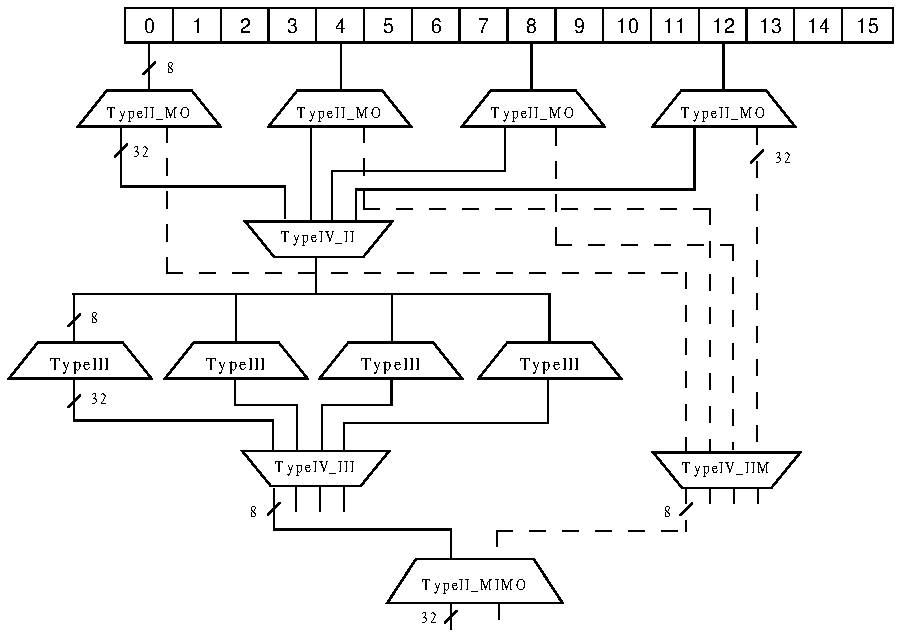
\includegraphics[width=7cm]{./pics/DCA_R12.pdf}
		\caption{Lookup sequence from the first column in the first round to the first byte at the second round. (Solid line represents the data flow of masked values while the dotted line denotes the one of mask used.)}
	\end{figure}
}

\frame
{
	\begin{figure}
		\centering
		\begin{minipage}[b]{0.35\textwidth}
			%\centering
			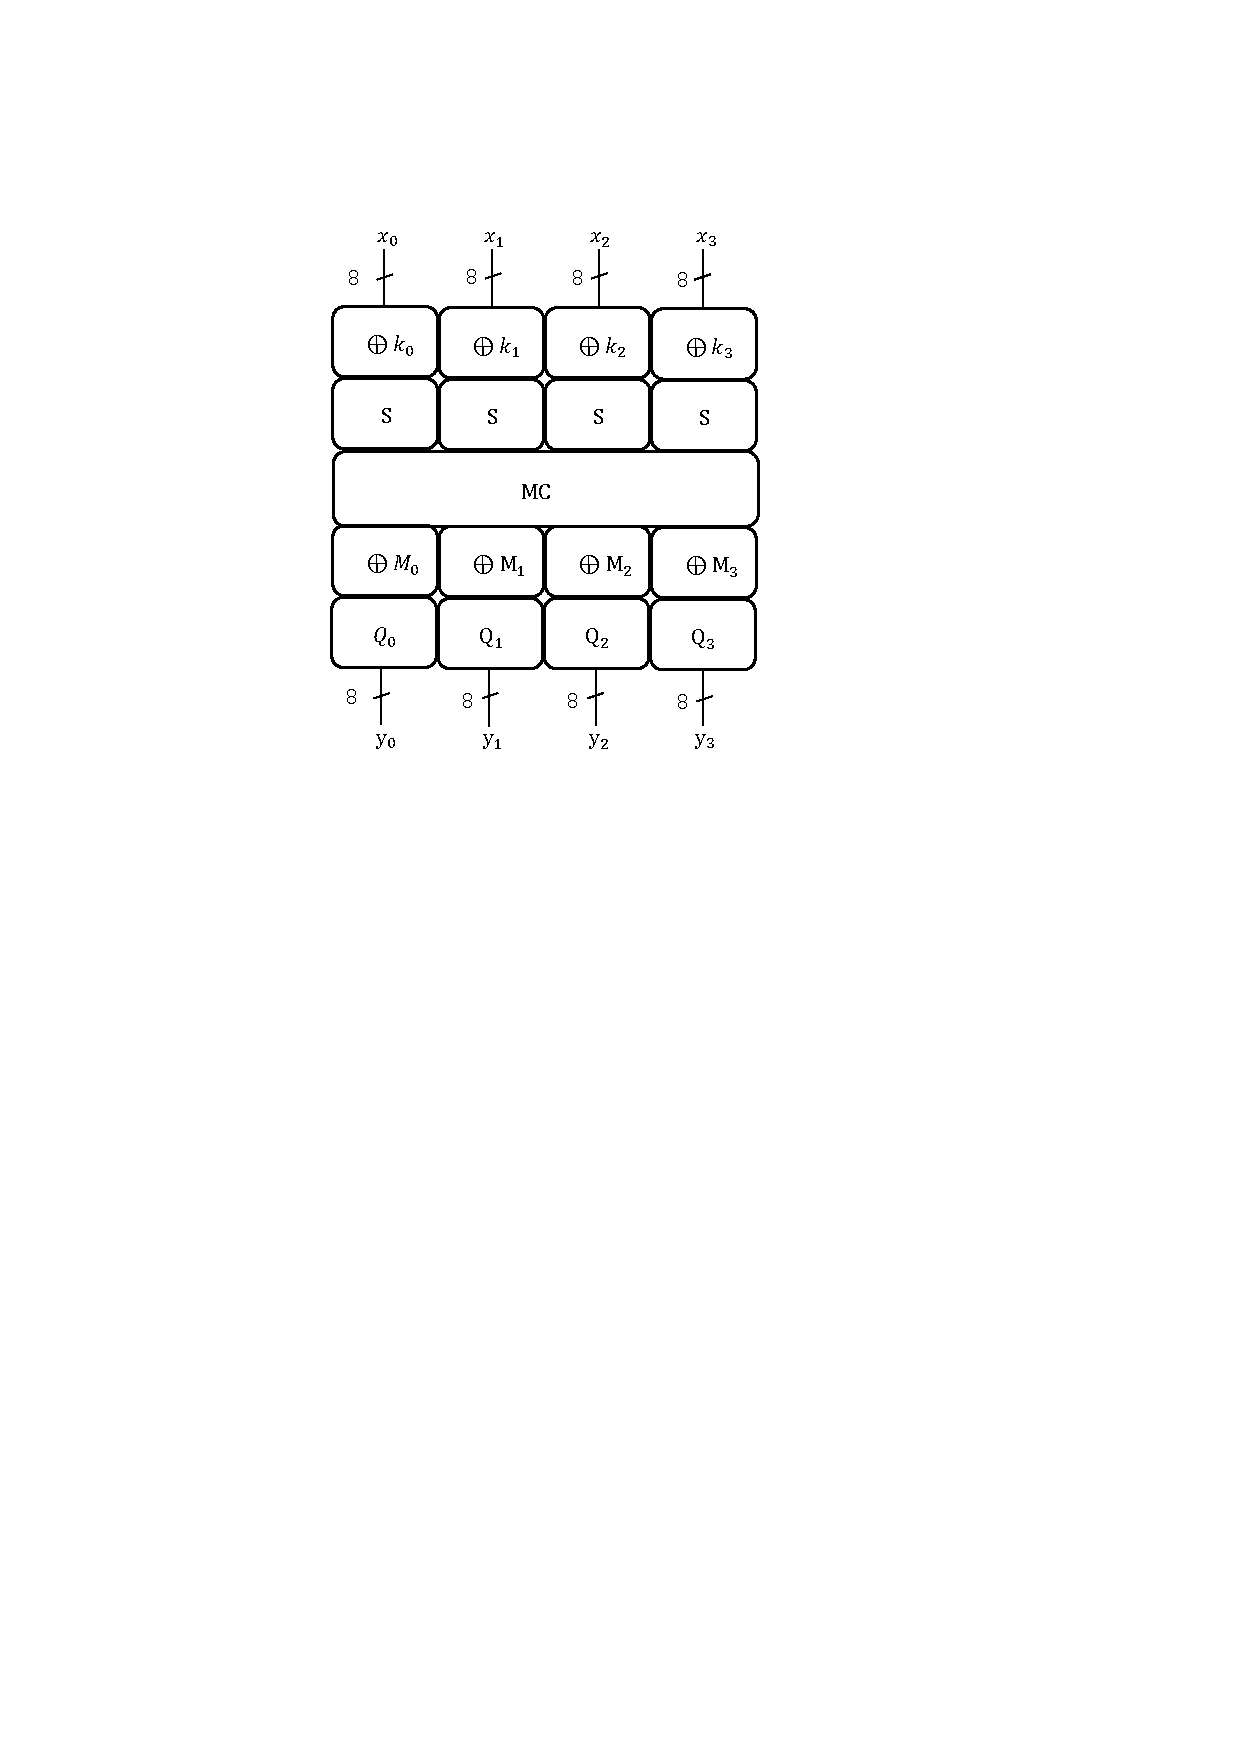
\includegraphics[width=4.5cm]{./pics/DCA_comR12.pdf}
			\caption{Composition of the encoded masked 1-st round output (solid line).}
		\end{minipage}%
		\hspace{0.1\textwidth}%
		\begin{minipage}[b]{0.35\textwidth}
			%\centering
			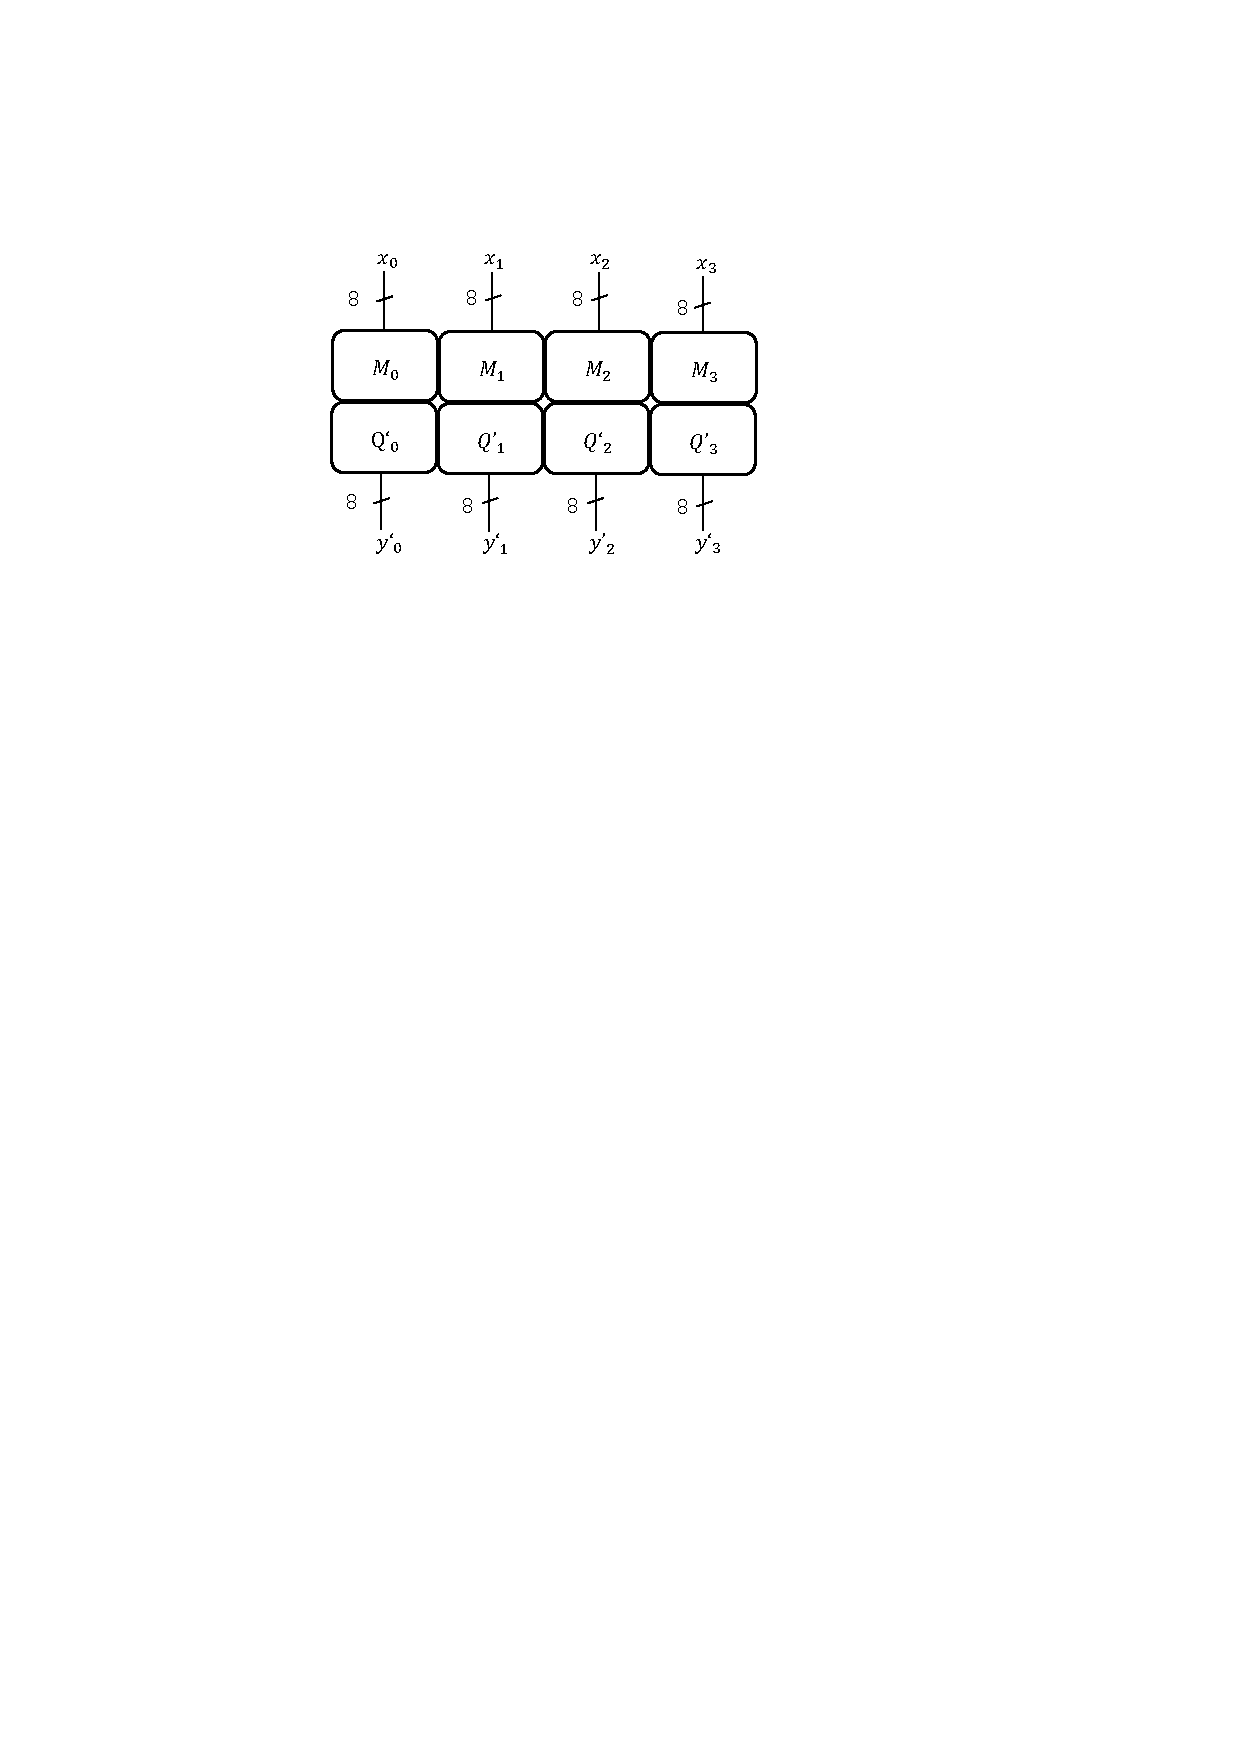
\includegraphics[width=4.5cm]{./pics/DCA_comR12M.pdf}
			\caption{Composition of the encoded mask in 1-st round (dotted line).}
		\end{minipage}
	\end{figure}
}

\frame
{
	The encoded and masked 1-st round functions are shown in below.
	\[
	\begin{aligned}
	y_i(x_0,x_1,x_2,x_3)=&Q_i\circ(mc_{i,0}\cdot S[x_0\oplus k_0]\oplus mc_{i,1}\cdot S[x_1\oplus k_1]\\
	&\oplus mc_{i,2}\cdot S[x_2\oplus k_2]\oplus mc_{i,3}\cdot S[x_3\oplus k_3]\oplus M_i).
	\end{aligned}
	\]
	The encoded output of mask table can be represent as follows.
	\[y'_i(x_0,x_1,x_2,x_3)=Q'_i\circ(M_i),\]
	where $M_i$ denotes the mask used, $mc_i$ denotes the \textbf{MixColumns} coefficient, $0\leq i\leq 3$ denote the byte index of the column.
}

\frame
{
	Note that $x_0||x_1||x_2||x_3\ \in \mathbb{F}_{2}^{32}$, $M_i$ take all the values in $\mathbb{F}_{2}^{8}$. One can sort the inputs by the identical output $y'_i$ of mask table (e.g., get the input set $\mathcal{W}=\{x|y'(x)=c,x\in\mathbb{F}_{2}^{32}\}$, where $c$ is a constant).
	\\[2ex]
	In this way, for any input $x\in S$, the mask used of $y(x)$ is a constant.
	
}

\frame
{
	The detailed attack can be represented by the following steps.
	\begin{itemize}	
		\item Collecting the plaintexts to form the set $\mathcal{W}$ which have the same output of $y'_0$ by enumerating the first two bytes of the inputs and fixing the other bytes of $y'_0$ (e.g., $y'_0(x_0,x_1,0,0)$).
		\item Collecting the bit traces $\upsilon$ which include the values of the outputs of $y_0$ by choosing the plaintexts in $\mathcal{W}$.
	\end{itemize}
}

\frame
{
	\begin{itemize}
		\item Selecting the XOR of the first two outputs of MixColumns as the hypothetical value $b$, that is
		\begin{displaymath}
		b=mc_{i,0}\cdot S(x_0\oplus k'_0)\oplus mc_{i,1}\cdot S(x_1\oplus k'_1),
		\end{displaymath}
		where $k'_0$ and $k'_1$ are key guess.
		\item Mounting the DCA attack on analyzing the correlation between $\upsilon$ and $b$ to recover $k_0$ and $k_1$.
	\end{itemize}
}

\frame
{ 
	\frametitle{Work Factor of Adaptive DCA on Improved Masking}
	After the reverse engineering, the experimental results show that, 
	\begin{enumerate}[1.]
		\item at least about 3,265 times can recover four 2-byte subkeys of the first round,
		\item totally at least about 6,530 times encryption can extract the 16-byte first-round key.
	\end{enumerate}
}

\subsection{Adaptive DFA on Table Redundancy WBAES}
\frame
{
	\frametitle{Table Redundancy Method for Protecting Against DFA}
	In 2019, Lee \textit{et al.} [eprint 2019/959] prorosed a table redundancy scheme based on Chow \textit{et al.}'s white-box AES for protecting against DFA.
	\\[2ex]
	Table redundancy method uses multiple branches of look-up tables for the target rounds (Round 7, 8, and 9) and xor the output to detect the modification.
}

\frame
{
	\frametitle{Different types of LUTs in Chow \textit{et al.}'s WBAES}
	\begin{figure}
		\centering
		\begin{minipage}[b]{0.3\textwidth}
			%\centering
			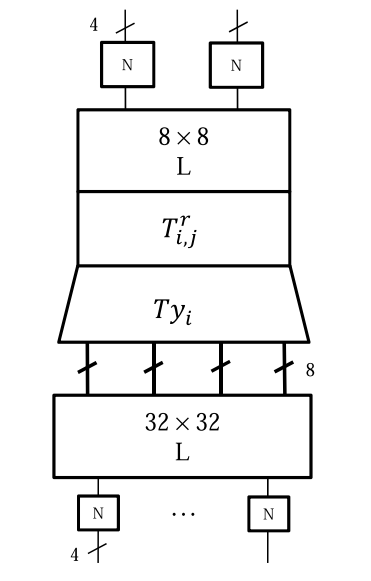
\includegraphics[width=3cm]{./pics/TMC.png}
			\caption{Type II: key-dependent T-boxes/$Ty_i$ table}
		\end{minipage}%
		\hspace{0.04\textwidth}%
		\begin{minipage}[b]{0.3\textwidth}
			%\centering
			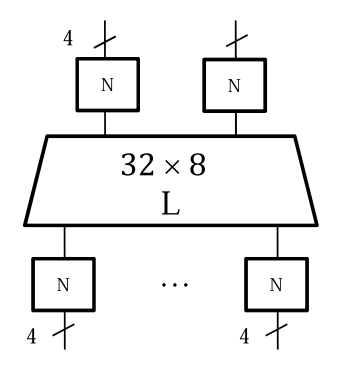
\includegraphics[width=3cm]{./pics/type3.png}
			\caption{Type III: compatibility of encodings
				between consecutive rounds}
		\end{minipage}
		\hspace{0.04\textwidth}%
		\begin{minipage}[b]{0.2\textwidth}
			%\centering
			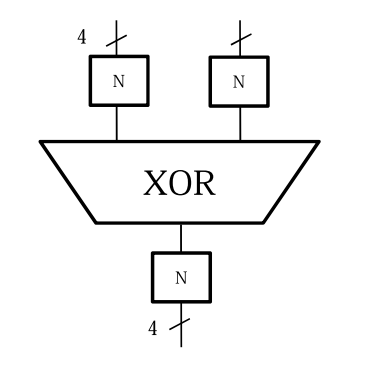
\includegraphics[width=2.7cm]{./pics/type4.png}
			\caption{Type IV: encoded nibble XOR table}
		\end{minipage}
	\end{figure}
}

\frame
{
	\begin{figure}
		\centering
		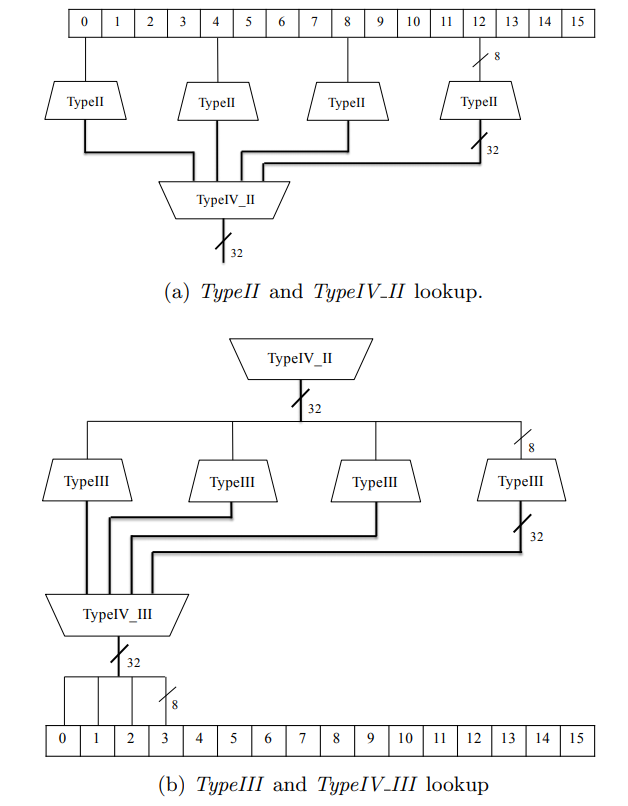
\includegraphics[width=5cm]{./pics/type234.png}
		\caption{An overview of \textit{TypeII}, \textit{TypeIII} and \textit{TypeIV} table lookups.}
	\end{figure}
}

\frame
{
	\frametitle{Table redundancy protection}
	The distribution of the redundant computation can be shown as four parts as follows.
	\begin{itemize}
		\item Sharing the look-up tables from Round 1 to 6.
		\item Transforming independently in parallel with two sets of look-up tables from Round 7 to \textit{TypeII} in Round 9.
		\item XOR (by a type of \textit{TypeIV}) the output of two redundant computations.
		\item Sharing the look-up tables from 9-th \textit{TypeIV\_II} to Round 10.
	\end{itemize}
}

\frame
{
	\begin{figure}
		\centering
		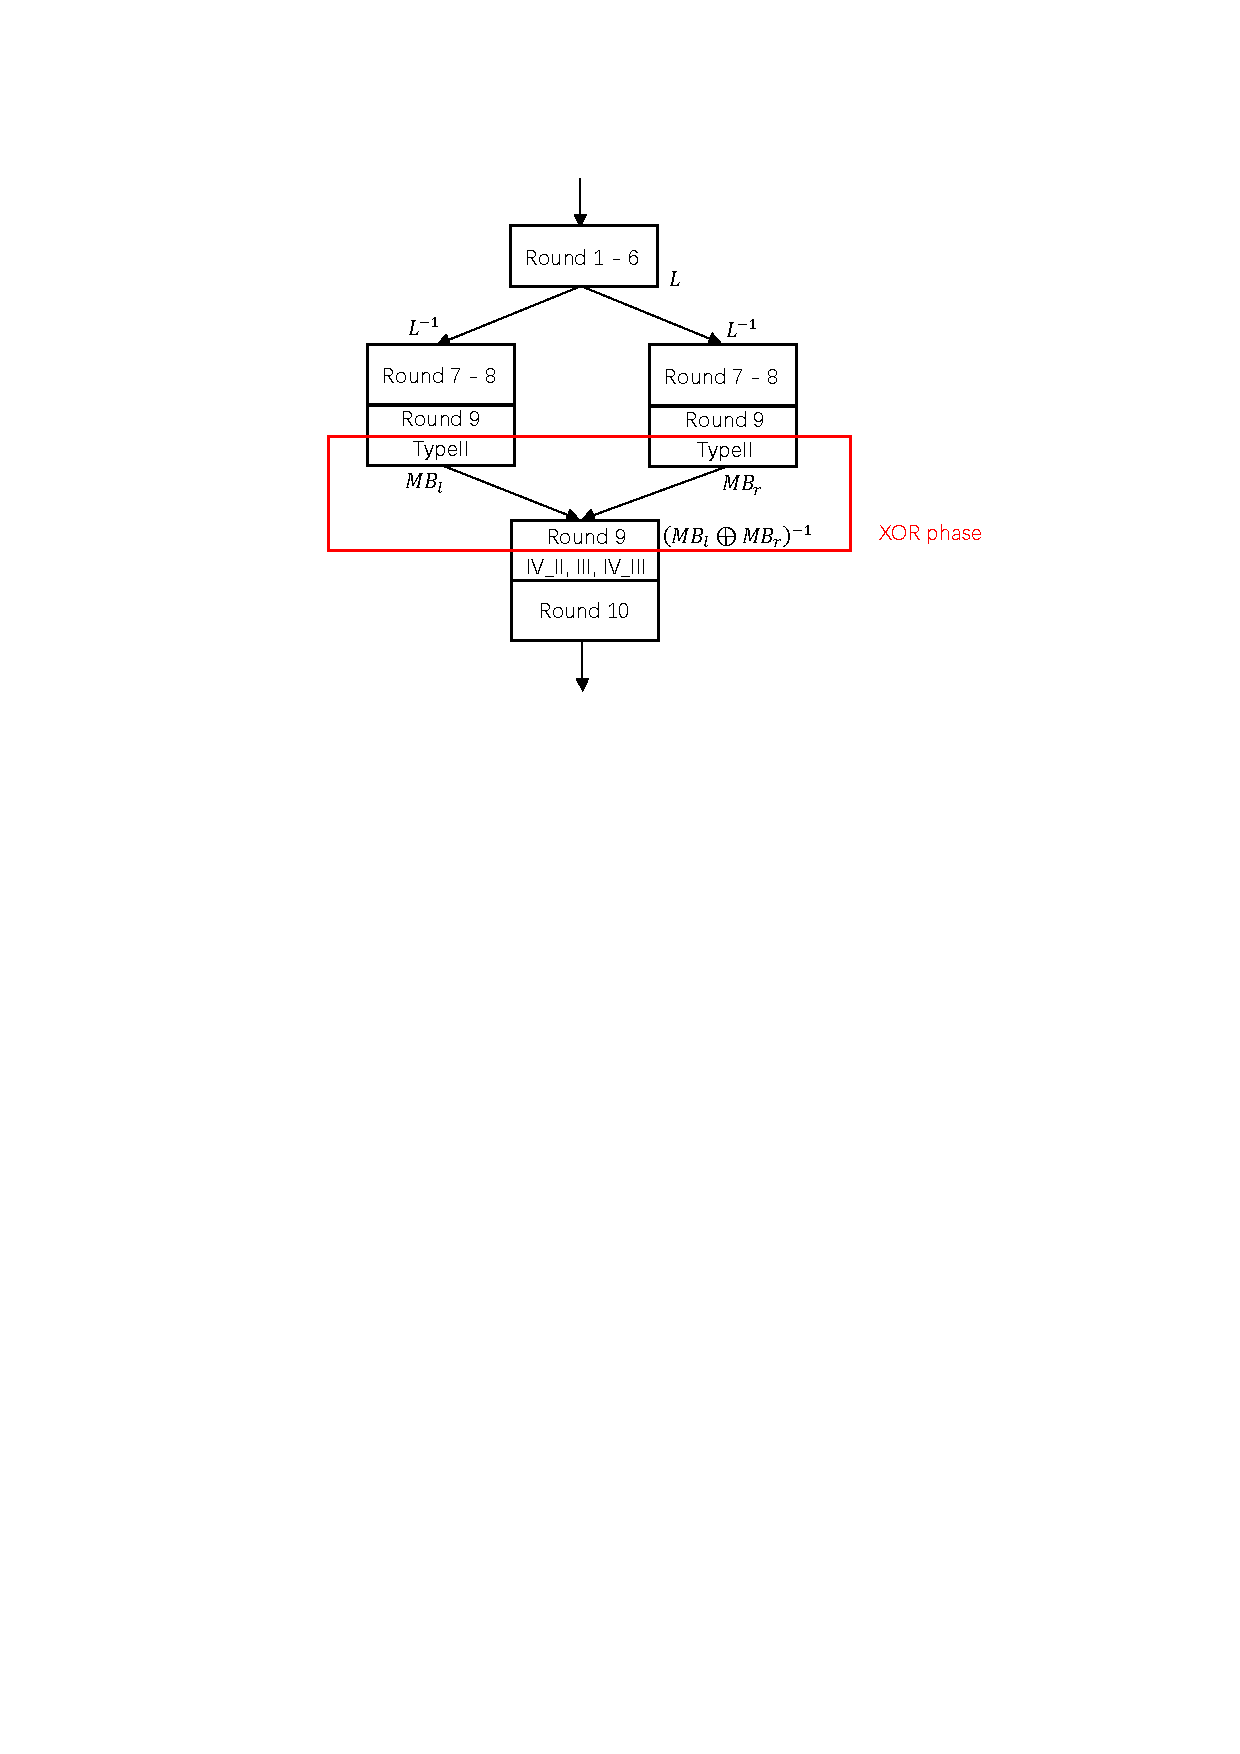
\includegraphics[width=8cm]{./pics/TRS1.pdf}
		\caption{The lookup sequence of table redundant scheme.}
	\end{figure}
}

\frame
{
	\begin{itemize}
		\item $MB_{l},\ MB_{r} \in \mathbb{F}_{2}^{32\times 32}$, the left and right 32-bit linear encoding.
		\item $x_{l},\ x_{r} \in \mathbb{F}_{2}^{32}$, the underlying state of 9-th \textit{TypeII} output.
	\end{itemize}
	The XOR phase can be shown as 
	\[MB_{l}\cdot x_{l} \oplus MB_{r}\cdot x_{r} = (MB_{l} \oplus MB_{r}) \cdot x,\ iff\ x_{l} = x_{r} = x.\]
	\\[2ex]
	The inverse Mixing Bijection $MB^{-1} \in \mathbb{F}_{2}^{32\times 32}$ in 9-th \textit{TypeIII} can be depicted as \[MB^{-1} = (MB_{l} \oplus MB_{r})^{-1}.\]
}
\frame{
	\frametitle{The 9-th round byte-fault model}
	\begin{columns}
		\column{.4\textwidth}
		\begin{figure}
			\centering
			% Requires \usepackage{graphicx}
			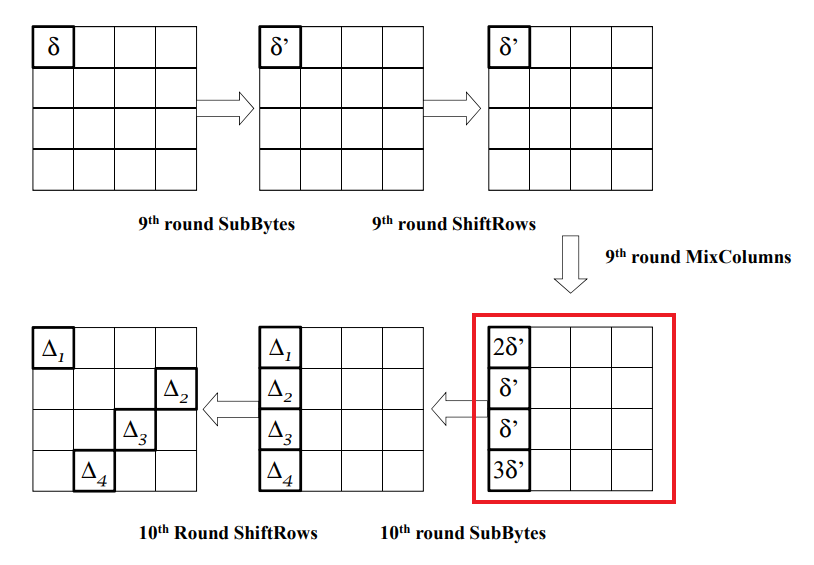
\includegraphics[width=4.5cm]{./pics/DFA_on_AES_1.png}
			\caption{The 9-th round faulty model of AES.}
		\end{figure}
		\column{.6\textwidth}
		\begin{itemize}
		\item $C_i$, fault-free ciphertexts.
		\item $C_i^{*}$, faulty ciphertexts.
		\item $k_i^{*}$, key candidates.
		\end{itemize}
		\begin{eqnarray}
		2\delta' = S^{-1}(C_{0}\oplus K_{0}^{*})\oplus S^{-1}(C_{0}^{*}\oplus K_{0}^{*}),\nonumber\\
		\delta' = S^{-1}(C_{7}\oplus K_{7}^{*})\oplus S^{-1}(C_{7}^{*}\oplus K_{7}^{*}),\nonumber\\
		\delta' = S^{-1}(C_{10}\oplus K_{10}^{*})\oplus S^{-1}(C_{10}^{*}\oplus K_{10}^{*}),\nonumber\\
		3\delta' = S^{-1}(C_{13}\oplus K_{13}^{*})\oplus S^{-1}(C_{13}^{*}\oplus K_{13}^{*}).\nonumber
		\end{eqnarray}
	\end{columns}
}

\frame{
	\frametitle{DFA on Table Redundancy Method}
	\begin{itemize}
		\item $x\in \mathbb{F}_{2}^{8}$, the fault-free unencoded state.
		\item $x^{*}\in \mathbb{F}_{2}^{8}$, the faulty one.
	\end{itemize}
	The XOR phase now can be shown as 
	\[\mathrm{MB}_{l}\cdot \mathrm{T/Ty_i}(x) \oplus \mathrm{MB}_{r}\cdot \mathrm{T/Ty_i}(x^{*}) \neq (\mathrm{MB}_{l} \oplus \mathrm{MB}_{r}) \cdot \mathrm{T/Ty_i}(x).\]
	\\[2ex]
	In this way, the decoding phase of $\mathrm{MB}$ cannot work in the following transformation and thus the faulty ciphertexts cannot be exploited for DFA attack.
}

\frame
{
	\frametitle{Adaptive DFA against Table Redundancy Method}
	\begin{itemize}
		\item $y_{l}, y_{r} \in \mathbb{F}_{2}^{8}$, an 8-bit input value of the two 9-th \textit{TypeII} respectively.
		\item $x \in \mathbb{F}_{2}^{8}$, an 8-bit underlying state of $y_{l}$ and $y_{r}$.
		\item $P_{l}, P_{r} \in \mathbb{F}_{2}^{8}$, an 8-bit input decoding.
	\end{itemize}
	For the decoding process of 9-th round input, we have
	\[x = P_{l}(y_{l}) = P_{r}(y_{r}).\]
}

\frame
{
	\begin{figure}
		\centering
		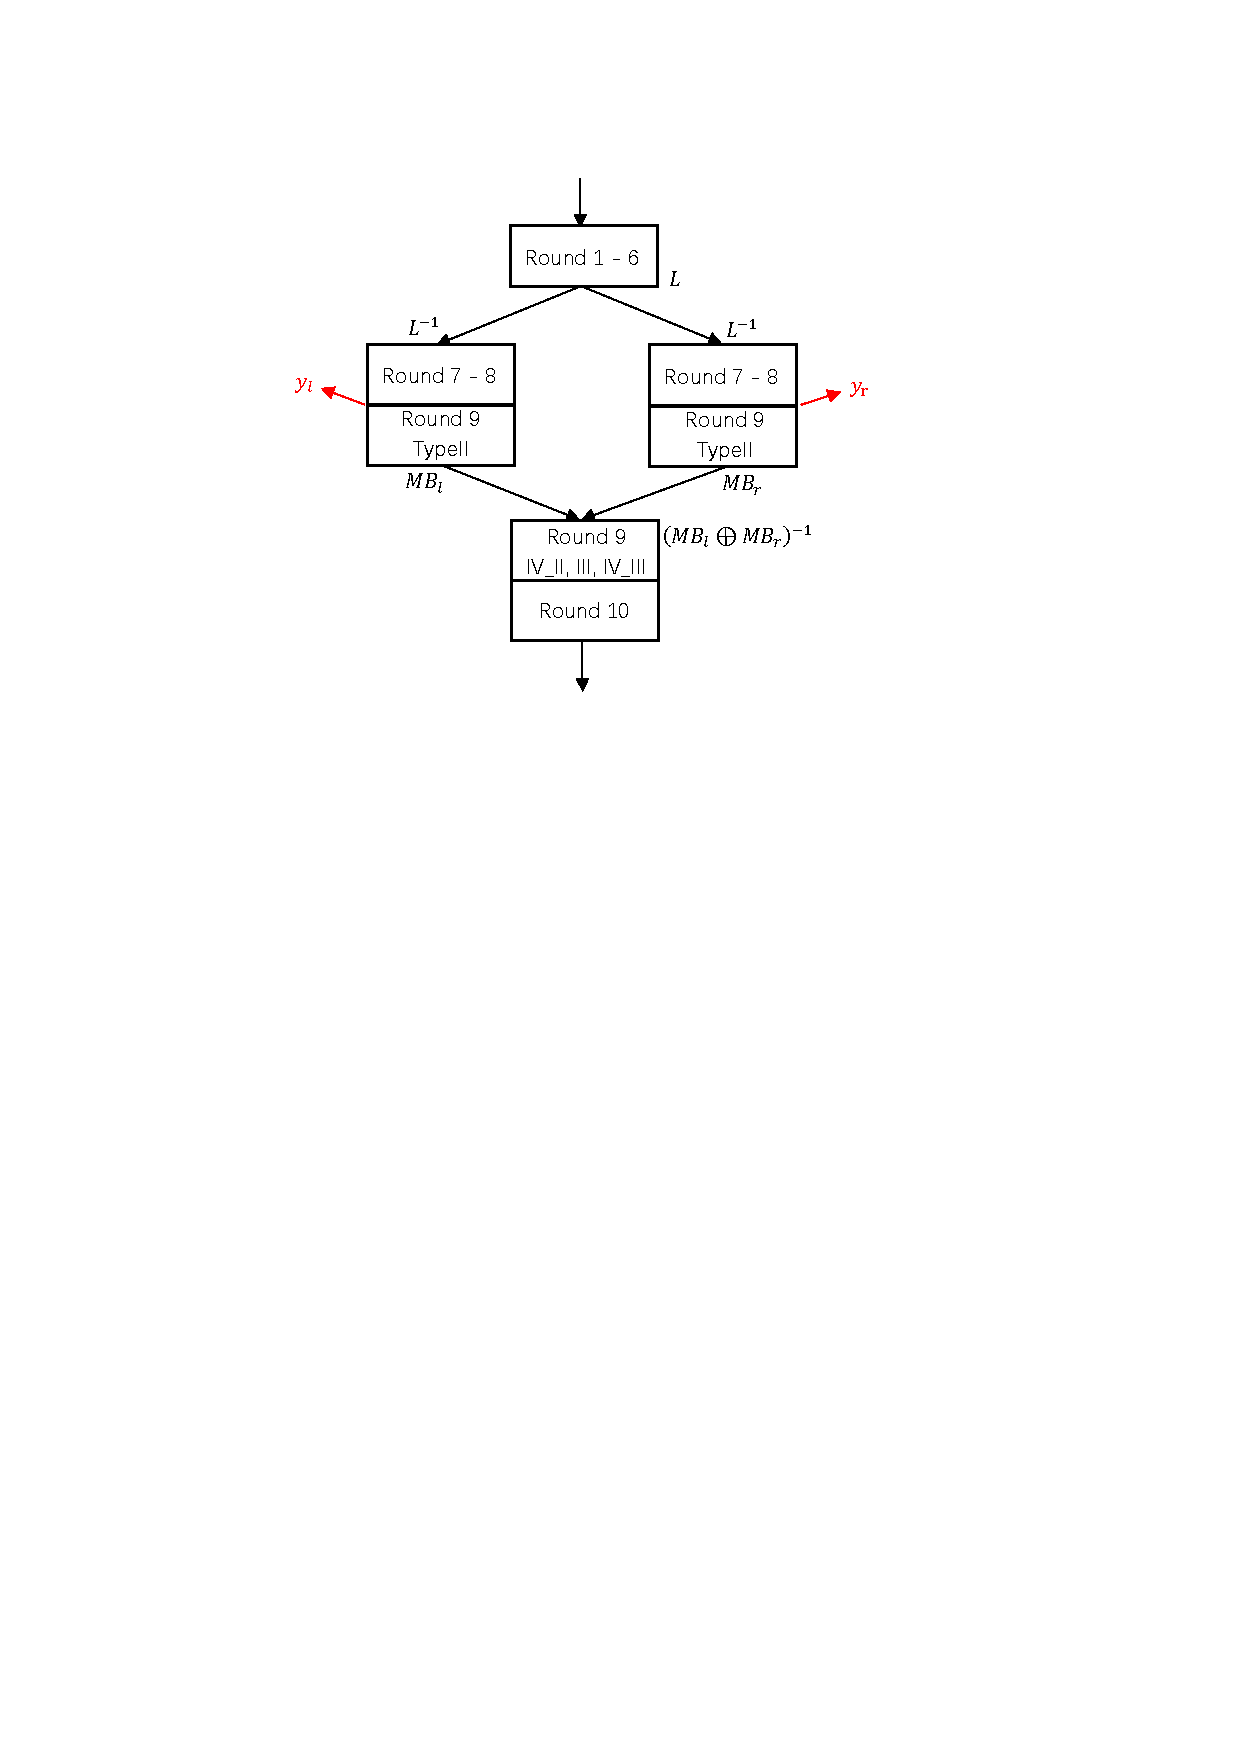
\includegraphics[width=8cm]{./pics/TRS2.pdf}
		\caption{The 9-th round input in the lookup sequence of table redundant scheme.}
	\end{figure}
}

\frame
{
	Since $x$ take 256 different values, the 256 pairs of each ($y_{l},y_{r}$) can be collected. 
	\\[2ex]
	Let $\mathcal{T}$ be a set of pairs values, such that
	\[\mathcal{T}=\{(y_{l},y_{r})\ |\ y_{l} \in \mathbb{F}_{2}^{8},\ y_{r} \in \mathbb{F}_{2}^{8}\}\ with\ \#\mathcal{T}=256.\]
	\\[2ex]
	Replacing the intermediate pairs ($y_{l},y_{r}$) with the other pairs in $\mathcal{T}$ can induce the faults at 9-th input.
}

\frame
{
	The injection on the entry of the 9-th round can be concluded by the following steps.
	\begin{itemize}
		\item Collecting the pairs values of $\mathcal{T}$ by repeatedly running the cryptographic program with random plaintexts.
		\item Getting a fault-free cipertext with a chosen plaintext $P$.
		\item Replacing the ($y_{l},y_{r}$) with other pairs in $\mathcal{T}\backslash(y_{l},y_{r})$ and collecting the faulty ciphertexts by repeatedly running the cryptographic program with $P$.
		\item Using the 9-th round byte-fault model to perform the analysis between the fault-free and faulty ciphertexts.
	\end{itemize}
}




\subsection{Open problem: Adaptive DCA on the CHES 2021 Proposal}
\frame
{ 
	\frametitle{Adaptive DCA on the CHES 2021 Proposal}
	In CHES 2021, Seker \textit{et al.} proposed a masking scheme for resisting DCA and Algebraic DCA attacks.
	\\[2ex]
	\begin{itemize}
		\item $\tilde{x}_0,...,\tilde{x}_d,x_1,...,x_n$, shares of sensitive variable $x$.
		\item Making: $x=\prod_{j=0}^{d}\tilde{x}_j\oplus \sum_{i=1}^{n}x_i$.
	\end{itemize}
}
\frame
{ 
	Note that,
	\[Pr(\prod_{j=0}^{d}\tilde{x}_j=0)=1-(\frac{1}{2})^{d+1}.\]
	\\[2ex]
	Hence, $x=\sum_{i=1}^{n}x_i$ with a high probability for the increasing $d$, there exists $n$ nodes that are linearly correlated with a predictable vector. 
	\\[2ex]
	An Adaptive DCA attacker can mount the higher-order DCA attack [Bogdanov \textit{et al.} 2019] directly on the circuit after the reverse engineering effort.
	\\[2ex]
	But how about decoding the key shares with the ability of a white-box attacker?
}

\section{Conclusion}

\frame{
\frametitle{The practical perspective of white-box security}
Since the secret values are the most important in the white-box security model. A white-box cryptography should provide the following security properties.

\begin{itemize}
\item \textbf{Algorithm level: \textcolor{red}{Key recovery}.}

\item \textbf{Module level: Function integrity.}

\item \textbf{System level: Code lifting}

\end{itemize}
}

\frame{
\frametitle{}
For symmetric-key algorithms, they might be used for message authentication, data encryption/decryption and pseudorandom number generating. According to these different usages, the security requirements for the implementations of those cryptographic algorithms are diverse. Considering this diversity, we define a practical security notion for white-box cryptography as follows.

\begin{itemize}
\item \textbf{Key integrity.}

\item \textbf{Key confidentiality.}

\item \textbf{Key equivalence.}
\end{itemize}

}

\frame
{
\frametitle{Conclusion}

\begin{itemize}
\setlength{\itemsep}{12pt}
\item Security notions and definitions for white-box cryptography still need precise analysis.

\item Only key extraction might not suitable for some applications, e.g., MACs and signatures.

\item A secure white-box cryptography does not imply the white-box security of a secrecy system based on it.
\end{itemize}

}

\frame
{
\begin{center}
\textbf{Thanks for your attentions!}
\end{center}
\begin{center}
\begin{tikzpicture}
    \node[anchor=south west,inner sep=0] (image) at (0,0) { 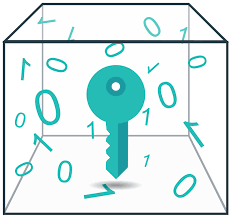
\includegraphics[width=4cm, height=4cm]{./pics/WBC_BG.png}};

    %\begin{scope}[x={(image.south east)},y={(image.north west)}]
        %\draw[help lines,xstep=.1,ystep=.1] (0,0) grid (1,1);
        %\foreach \x in {0,1,...,9} { \node [anchor=north] at (\x/10,0) {0.\x}; }
        %\foreach \y in {0,1,...,9} { \node [anchor=east] at (0,\y/10) {0.\y}; }
        %\draw[green, ultra thick, rounded corners] (0.24,0.18) rectangle (0.50,0.32);
    %\end{scope}
\end{tikzpicture}

\end{center}
}

\end{document}
